%========================================================================
% Chapter 3: System Design
%========================================================================
\chapter{System Design}

\section{System Description}

NepTube is a web-based video streaming application designed to provide an engaging platform for both content creators and viewers. Users can upload videos, create playlists, and manage their channels, while viewers can watch videos, comment, like or dislike, and subscribe to channels they enjoy. The platform integrates machine learning techniques, such as collaborative and content-based filtering, to deliver personalized video recommendations based on individual user preferences and viewing history.

Additionally, NepTube includes AI-powered tools that assist content creators by automatically generating video thumbnails, titles, and descriptions, helping improve content visibility and user engagement. The system is built with scalability and performance in mind \cite{choi2023qoe}, ensuring it can support a growing user base and content library. Focused on promoting Nepali and regional content, NepTube aims to offer a tailored and user-friendly experience for its audience.

\section{Flowchart}

An illustration of the logical flow and order of actions or steps in a system or process is called a flowchart. It represents numerous kinds of decisions, actions, inputs, outputs, and connectors using a variety of shapes and symbols. Workflows may be analyzed, communicated, and improved more easily when complicated processes are illustrated visually and simply via flowcharts. They are extensively used to visually map out processes and identify bottlenecks or areas for improvement in a variety of sectors, including software development, project management, business analysis, and problem-solving.

\subsection{User's Flowchart}

\begin{figure}[H]
\centering
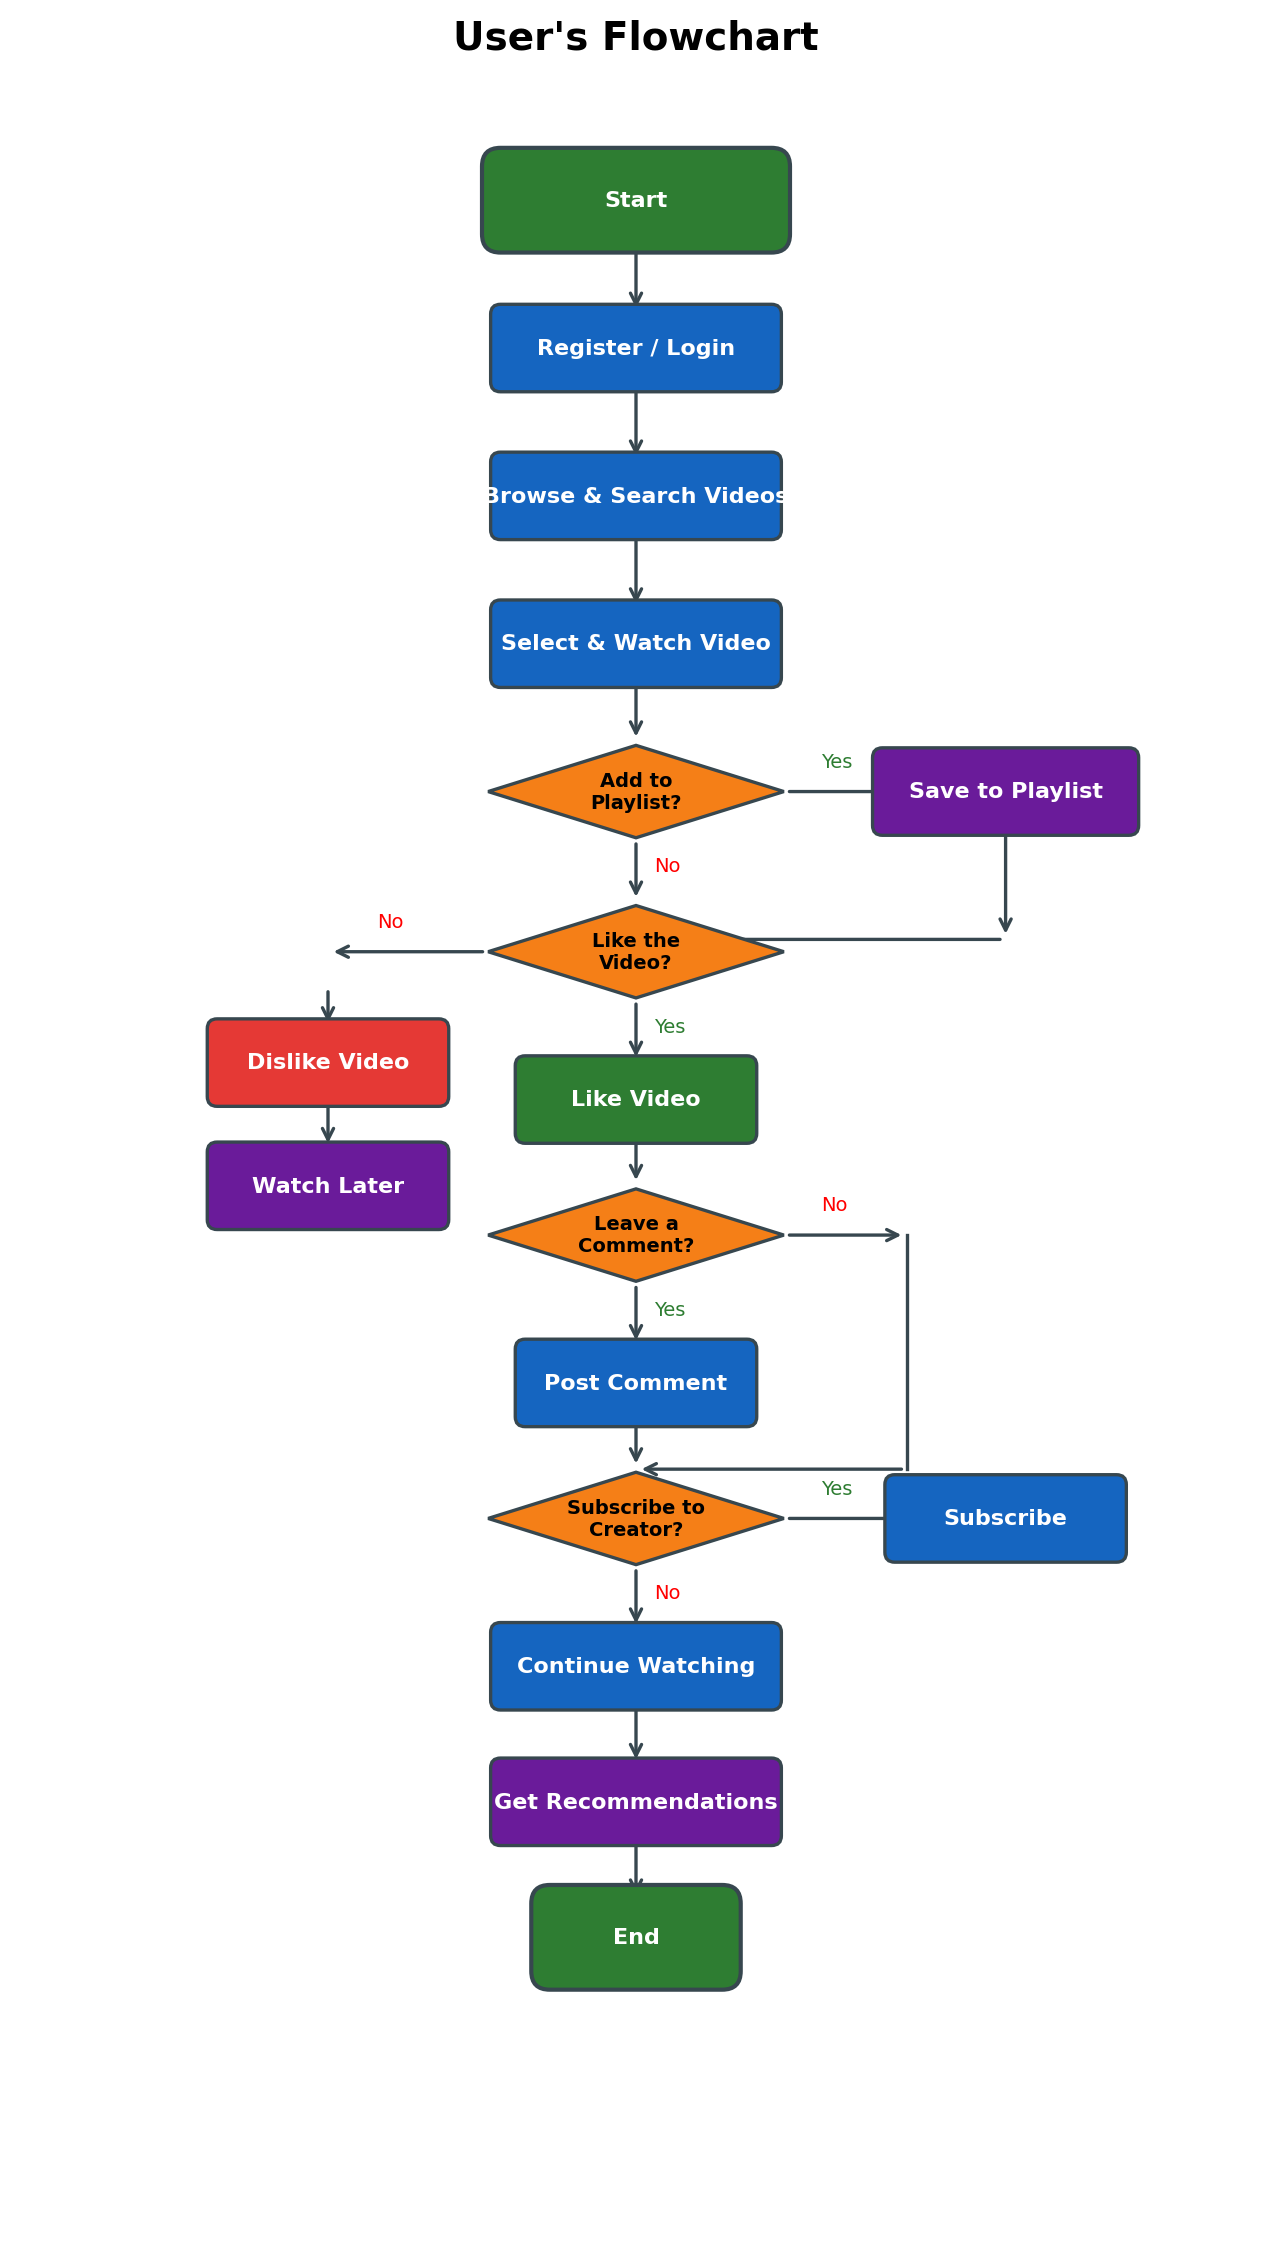
\includegraphics[width=0.85\textwidth]{images/user-flowchart.png}
\caption{User's Flowchart}
\label{fig:user-flowchart}
\end{figure}

The user's flowchart provides a clear and professional overview of how a user interacts with a video-sharing platform. It begins with the user registering or logging into the system, followed by browsing and searching for videos. Once a video is found, the user decides whether to add it to a playlist. If not, they evaluate whether they prefer the video. Based on their preference, the user may like or dislike the video. If they dislike it, they may choose to watch it later. If they like the video, they can choose to leave a comment. After commenting or not, the user is prompted to subscribe to the creator. Regardless of whether they subscribe, the user continues watching and receives recommendations for similar videos before the flow ends. This flowchart represents a typical interactive experience of a user engaging with content on the platform.

\subsection{Creator's Flowchart}

\begin{figure}[H]
\centering
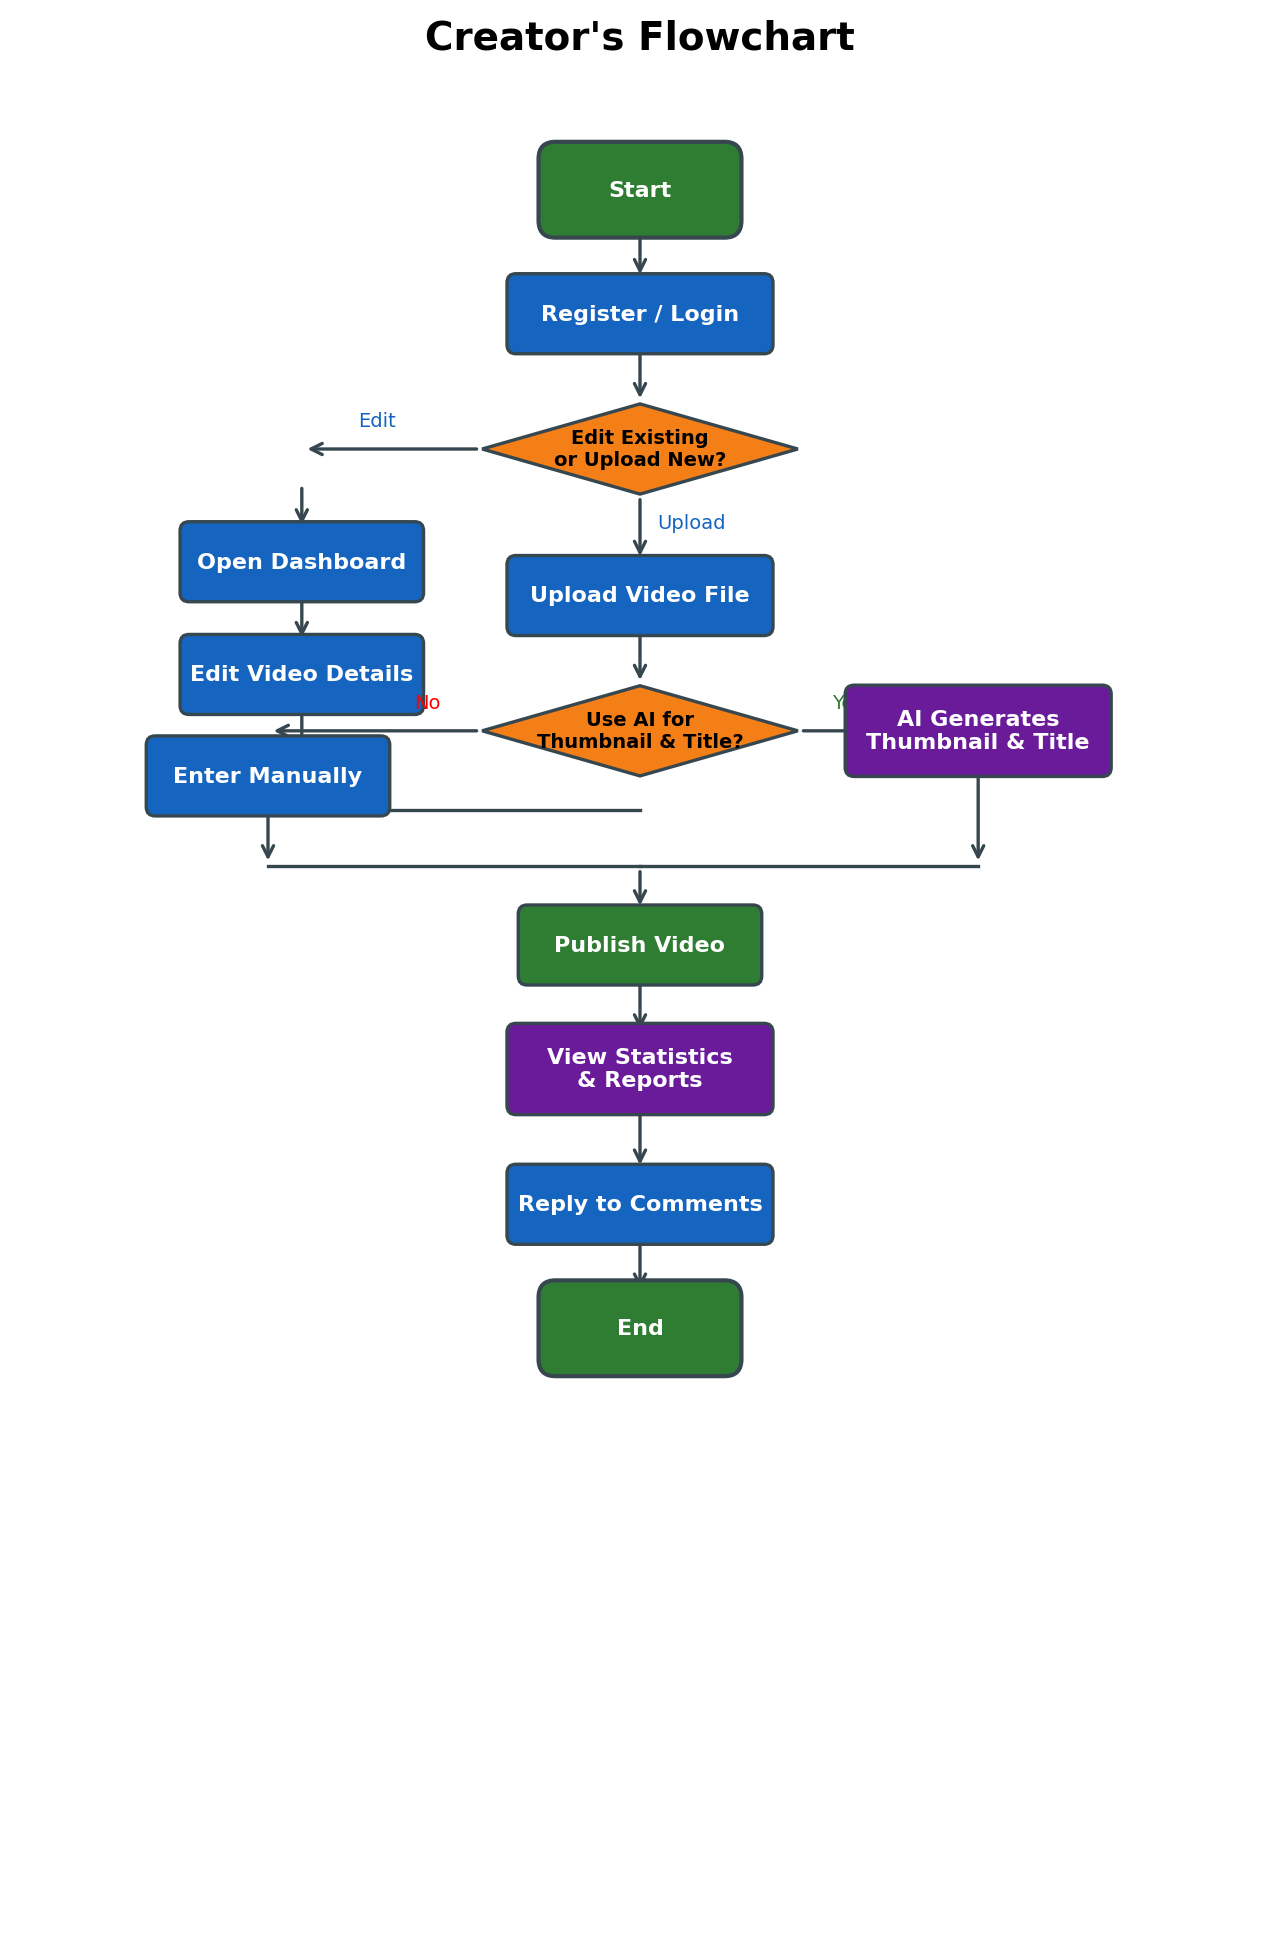
\includegraphics[width=0.85\textwidth]{images/creator-flowchart.png}
\caption{Creator's Flowchart}
\label{fig:creator-flowchart}
\end{figure}

The creator's flowchart provides a clear and organized overview of the steps a content creator follows on a video-sharing platform. It begins with the creator registering or logging into their account. After logging in, the creator can choose to either edit the details of a previously uploaded video or upload a new one. If they choose to edit, they are directed to the dashboard to make changes to existing content.

If the creator wants to upload a new video, they start by uploading the video file. Then, they are given the option to use AI-generated thumbnails and titles for the video or to enter them manually. This provides flexibility based on the creator's preference or need for convenience. Once the thumbnail and title are set---either through AI or manual input---the video is ready to be published.

After publishing, the creator can access detailed statistics and reports to track the performance of the video, such as views, likes, and comments. Finally, the creator can engage with the audience by replying to comments, which helps build a stronger connection with viewers. This flowchart effectively summarizes the content creation and management process, from uploading and editing to analyzing performance and engaging with the audience.

\section{Use Case Diagram}

Use case diagrams are a simple and effective way to show how different people interact with a system. They help us understand what the system is supposed to do by focusing on the users and their actions. Instead of getting into the technical details, these diagrams give a clear picture of the main features and how each user---like a customer, service provider, or admin---connects with them. This makes it easier for everyone involved, from developers to stakeholders, to stay on the same page and ensure the system meets real user needs.

\subsection{User's Use Case Diagram}

\begin{figure}[H]
\centering
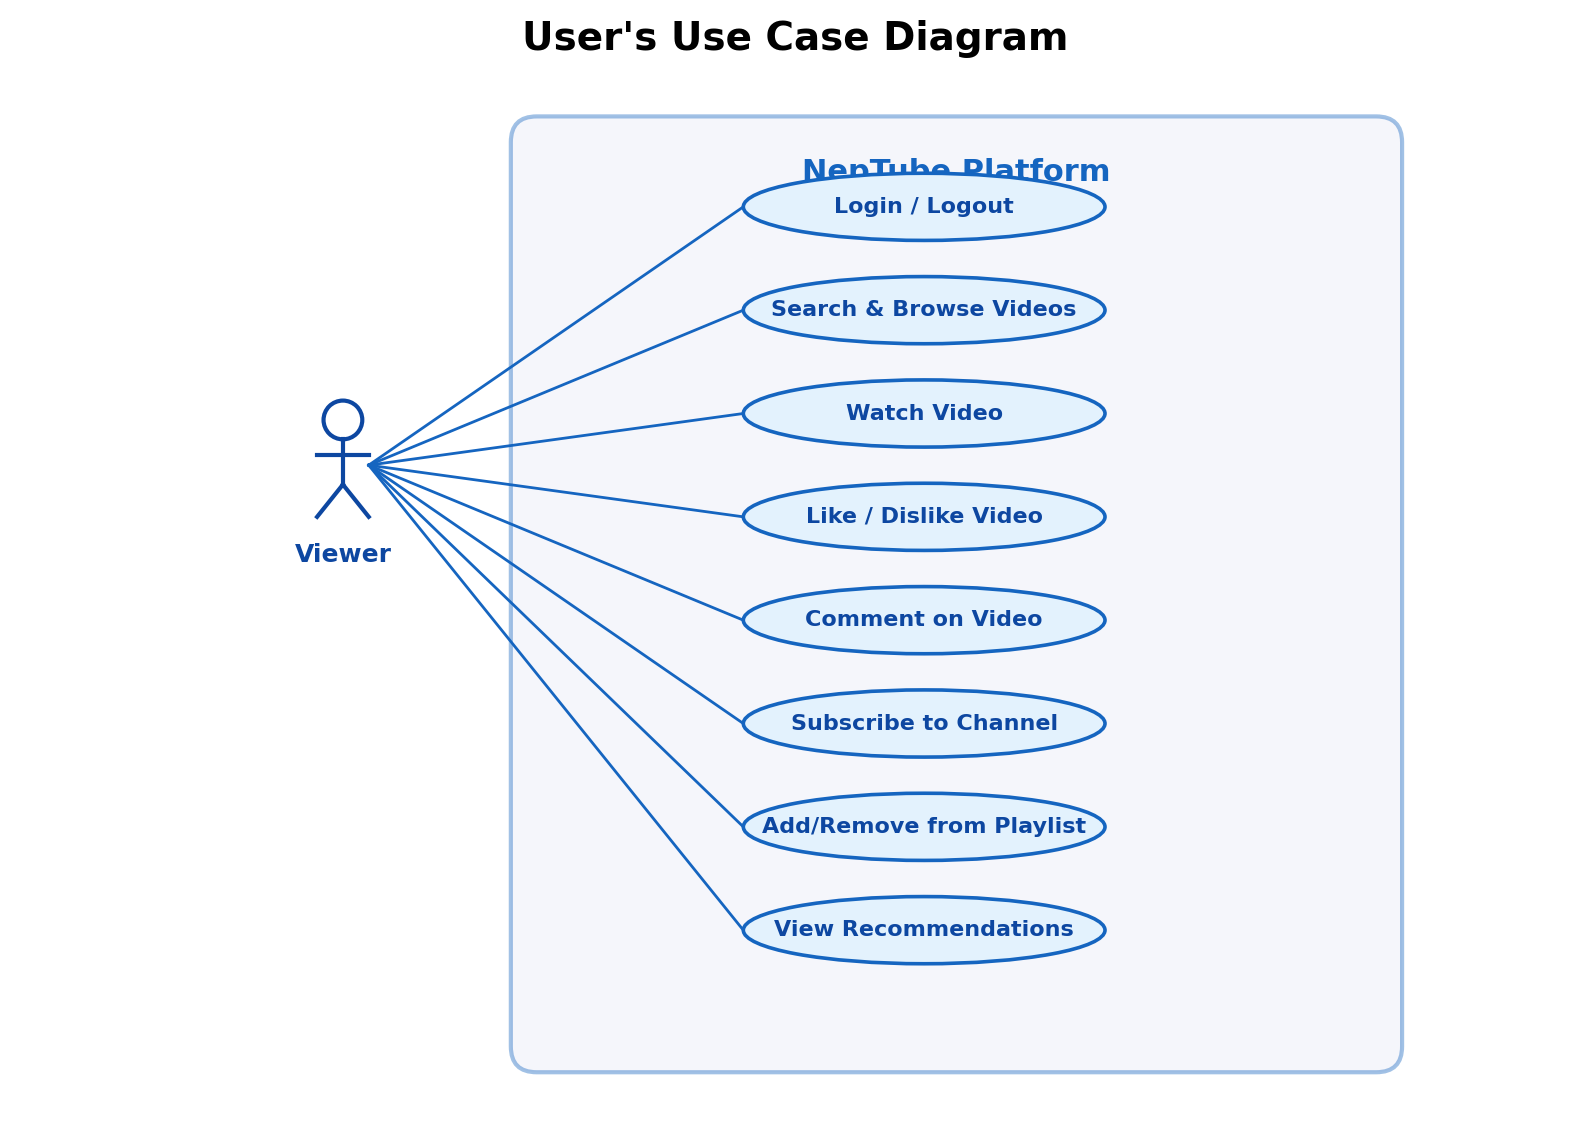
\includegraphics[width=0.85\textwidth]{images/user-usecase.png}
\caption{User's Use Case Diagram}
\label{fig:user-usecase}
\end{figure}

The use case diagram represents the interaction between a Viewer and a video streaming platform, outlining key functionalities for consuming and engaging with content. The Viewer begins by Logging in to access personalized features and can then Search or Browse Videos to discover content. Upon selecting a video, they can Watch it, with extended options to Like or Dislike and Comment, promoting user interaction. Viewers also have the ability to Delete their Comments, Subscribe to Channels for updates, and Add or Remove Videos from Playlists for easier organization. Additionally, the platform offers Recommendations based on viewing behavior. The session concludes with the Logout function. This diagram efficiently captures the essential actions a Viewer can take to interact with and personalize their experience on the platform.

\subsection{Creator's Use Case Diagram}

\begin{figure}[H]
\centering
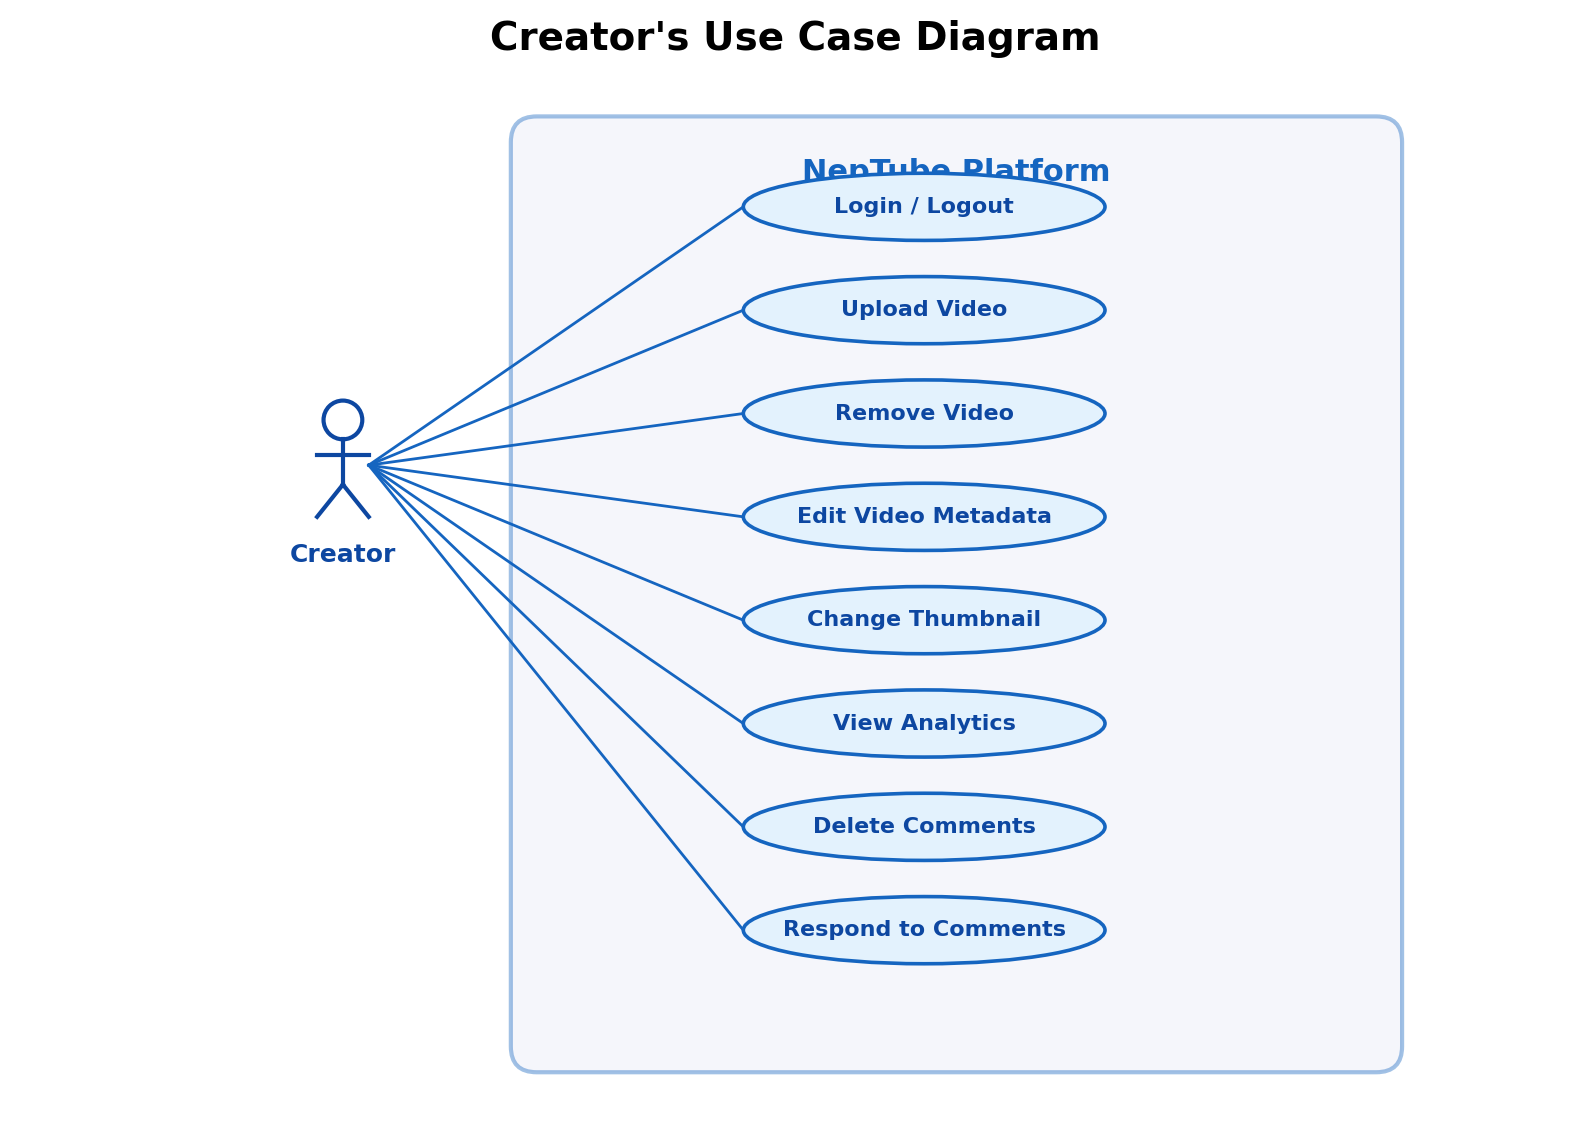
\includegraphics[width=0.85\textwidth]{images/creator-usecase.png}
\caption{Creator's Use Case Diagram}
\label{fig:creator-usecase}
\end{figure}

The use case diagram illustrates the interactions between a Creator and a video content platform, outlining the core functionalities available for managing video content. The Creator begins by performing a Login, enabling access to their account and content management tools. They can then Upload Video to share new content with viewers and Remove Video to delete existing content when necessary.

The Edit Video Metadata use case allows creators to modify details like titles, tags, and categories, while Change Thumbnail and Video Description support enhancing the visual and textual representation of the video. View Analytics enables creators to monitor video performance and audience engagement through data insights. In terms of community interaction, the Creator can Delete Comments that are inappropriate or irrelevant and Respond to Comments to engage directly with viewers. This diagram effectively summarizes the Creator's essential tools for content management, audience engagement, and performance tracking on the platform.

\subsection{Admin's Use Case Diagram}

\begin{figure}[H]
\centering
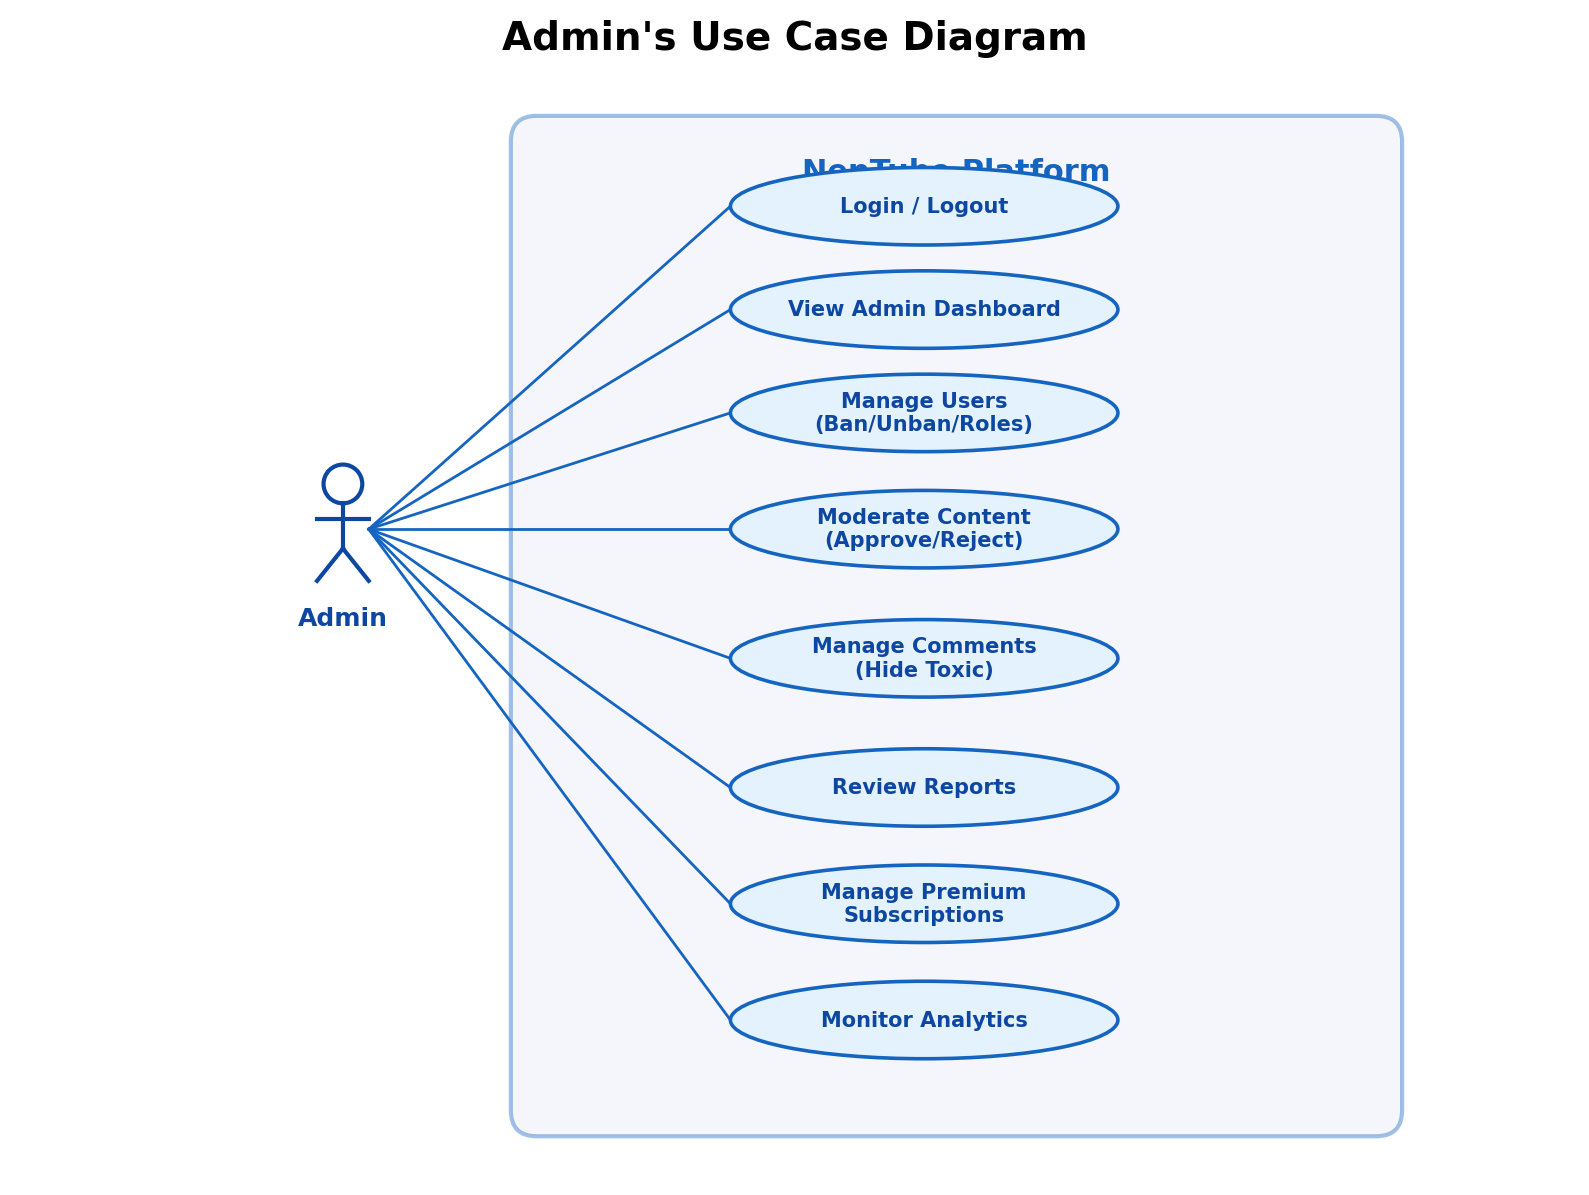
\includegraphics[width=0.85\textwidth]{images/admin-usecase.png}
\caption{Admin's Use Case Diagram}
\label{fig:admin-usecase}
\end{figure}

The admin's use case diagram illustrates the administrative functionalities available for platform management. The Admin can manage users (ban/unban, role changes, deletion), moderate content (approve/reject videos, review flagged content), manage comments (hide toxic comments, review reports), oversee premium subscriptions, and monitor platform analytics through the admin dashboard.

\section{Sequence Diagram}

Sequence diagrams help us visualize how different parts of a system communicate with each other over time. They show the step-by-step flow of messages between users and the system or between different parts of the system itself. This makes it easier to understand the exact order in which things happen. By breaking down the process into a timeline of interactions, sequence diagrams help developers plan, build, and troubleshoot the system more effectively.

\subsection{User's Sequence Diagram}

\begin{figure}[H]
\centering
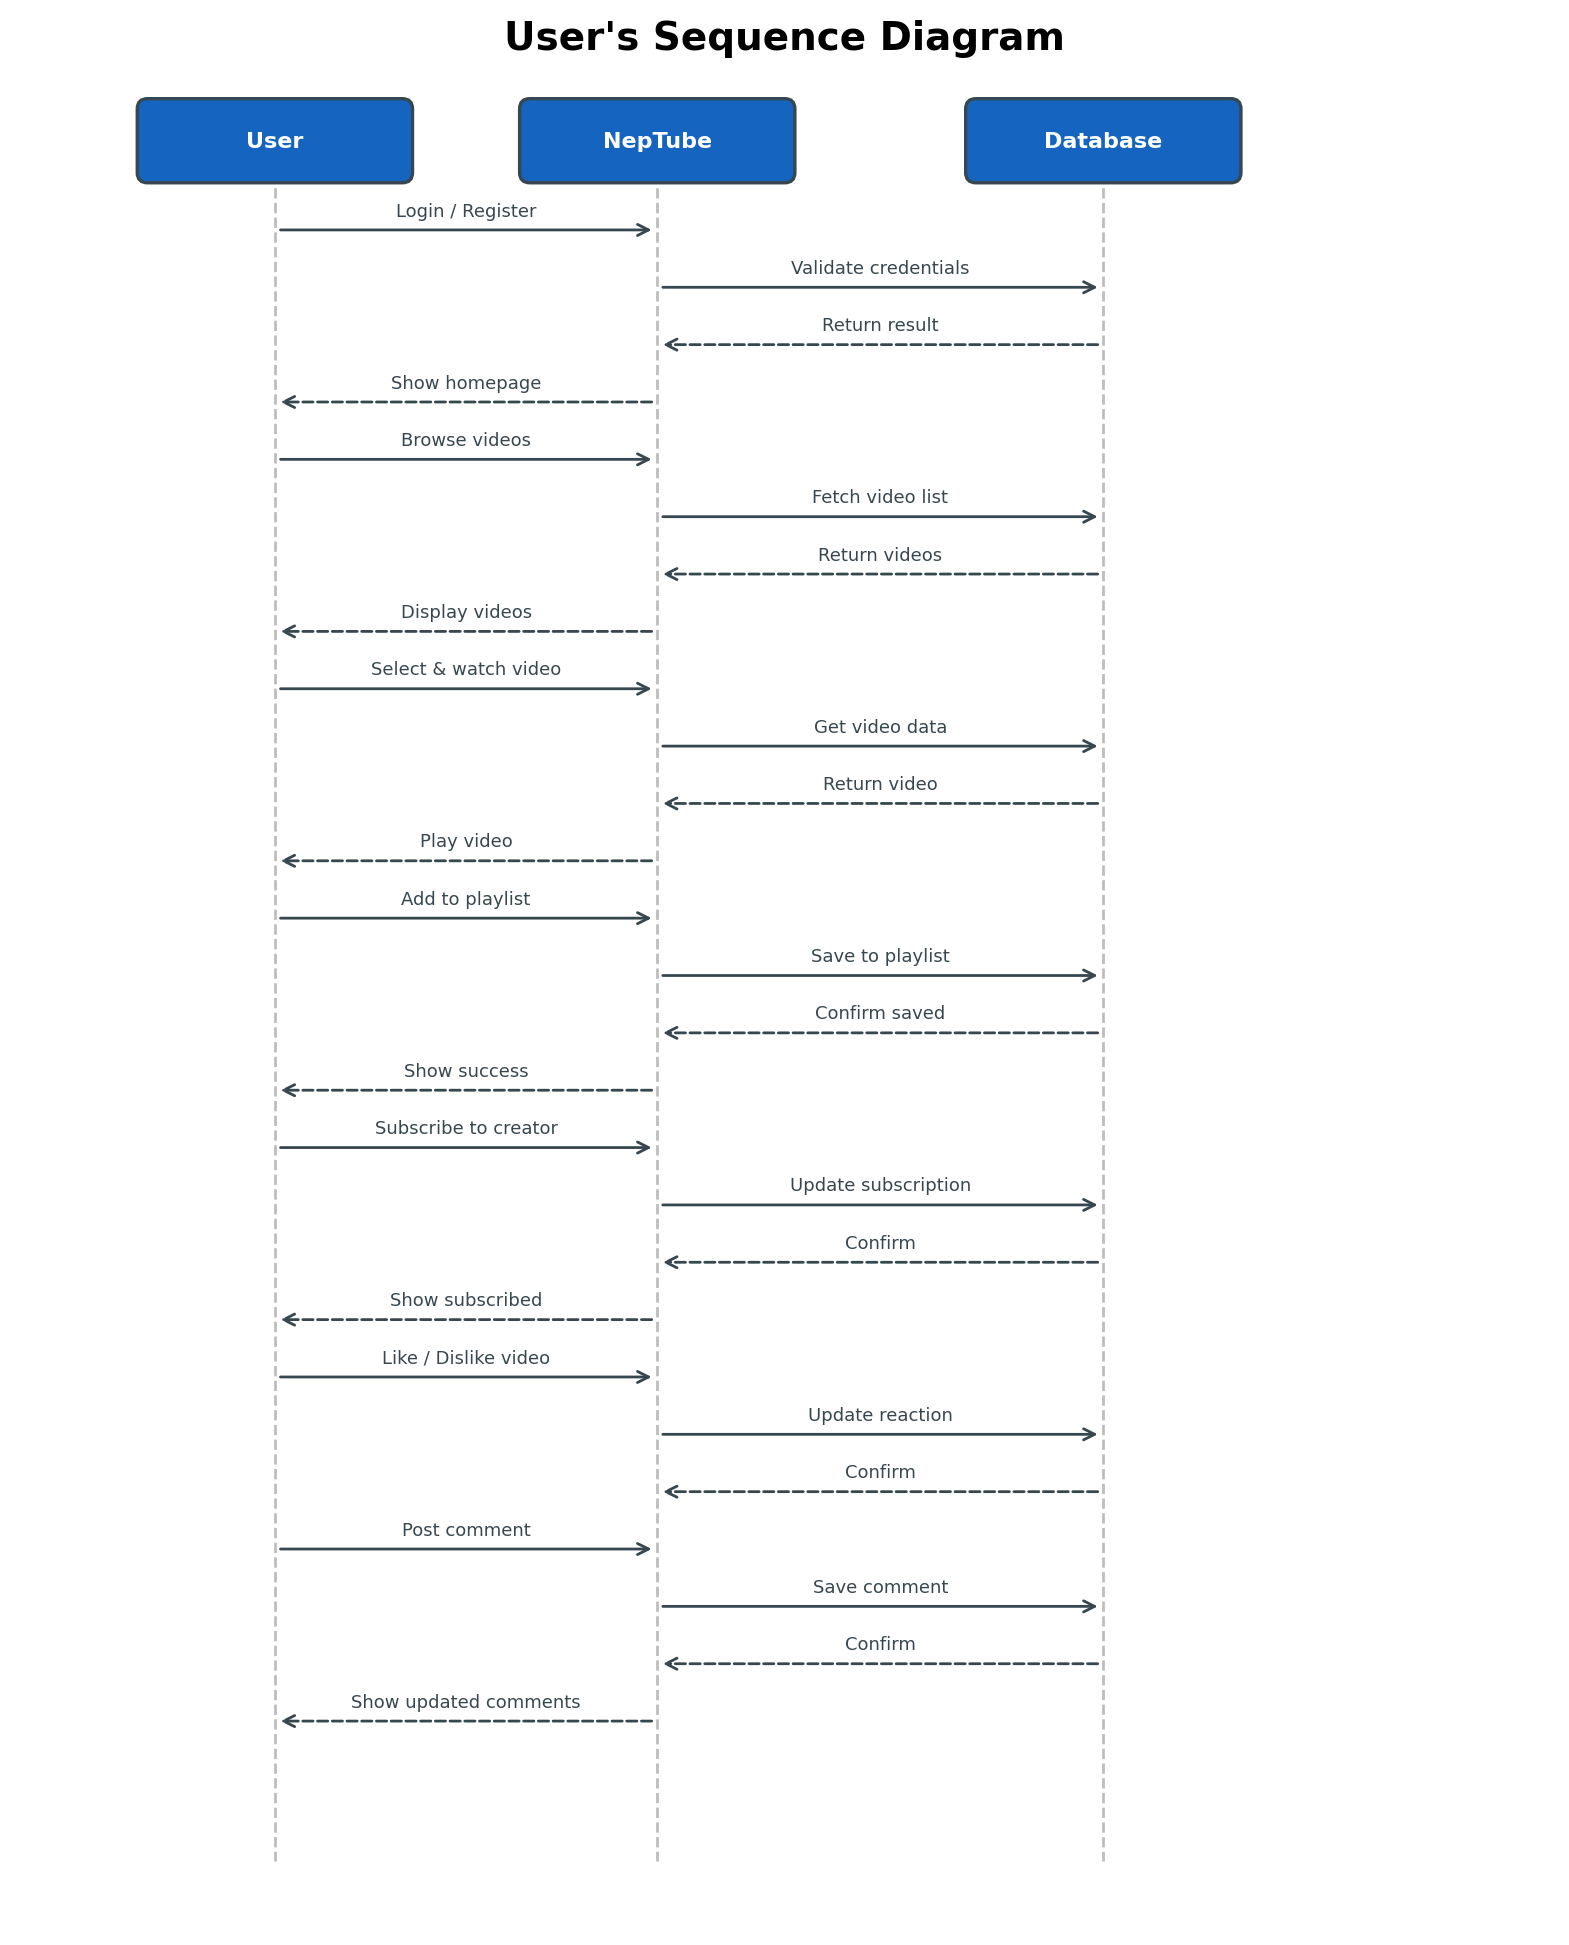
\includegraphics[width=0.9\textwidth]{images/user-sequence.png}
\caption{User's Sequence Diagram}
\label{fig:user-sequence}
\end{figure}

The user's sequence diagram illustrates the interaction between the user, the NepTube platform, and the database during various actions. It begins with the user logging in or registering, prompting NepTube to validate credentials with the database and return a success or failure message. Upon successful login, the homepage is shown, and the user browses videos. NepTube fetches the videos from creators, retrieves them from the database, and displays them to the user. When a video or channel is selected, NepTube retrieves the corresponding data and displays the video for playback. If the user adds the video to a playlist, it is saved in the database, confirmed, and a success message is shown. Subscribing to a creator updates the subscription list in the database, followed by a confirmation and display of a message. Liking or disliking a video updates the status in the database and shows a confirmation. Leaving or replying to a comment updates the comment section, confirms the update, and concludes with a success message.

\subsection{Admin's Sequence Diagram}

\begin{figure}[H]
\centering
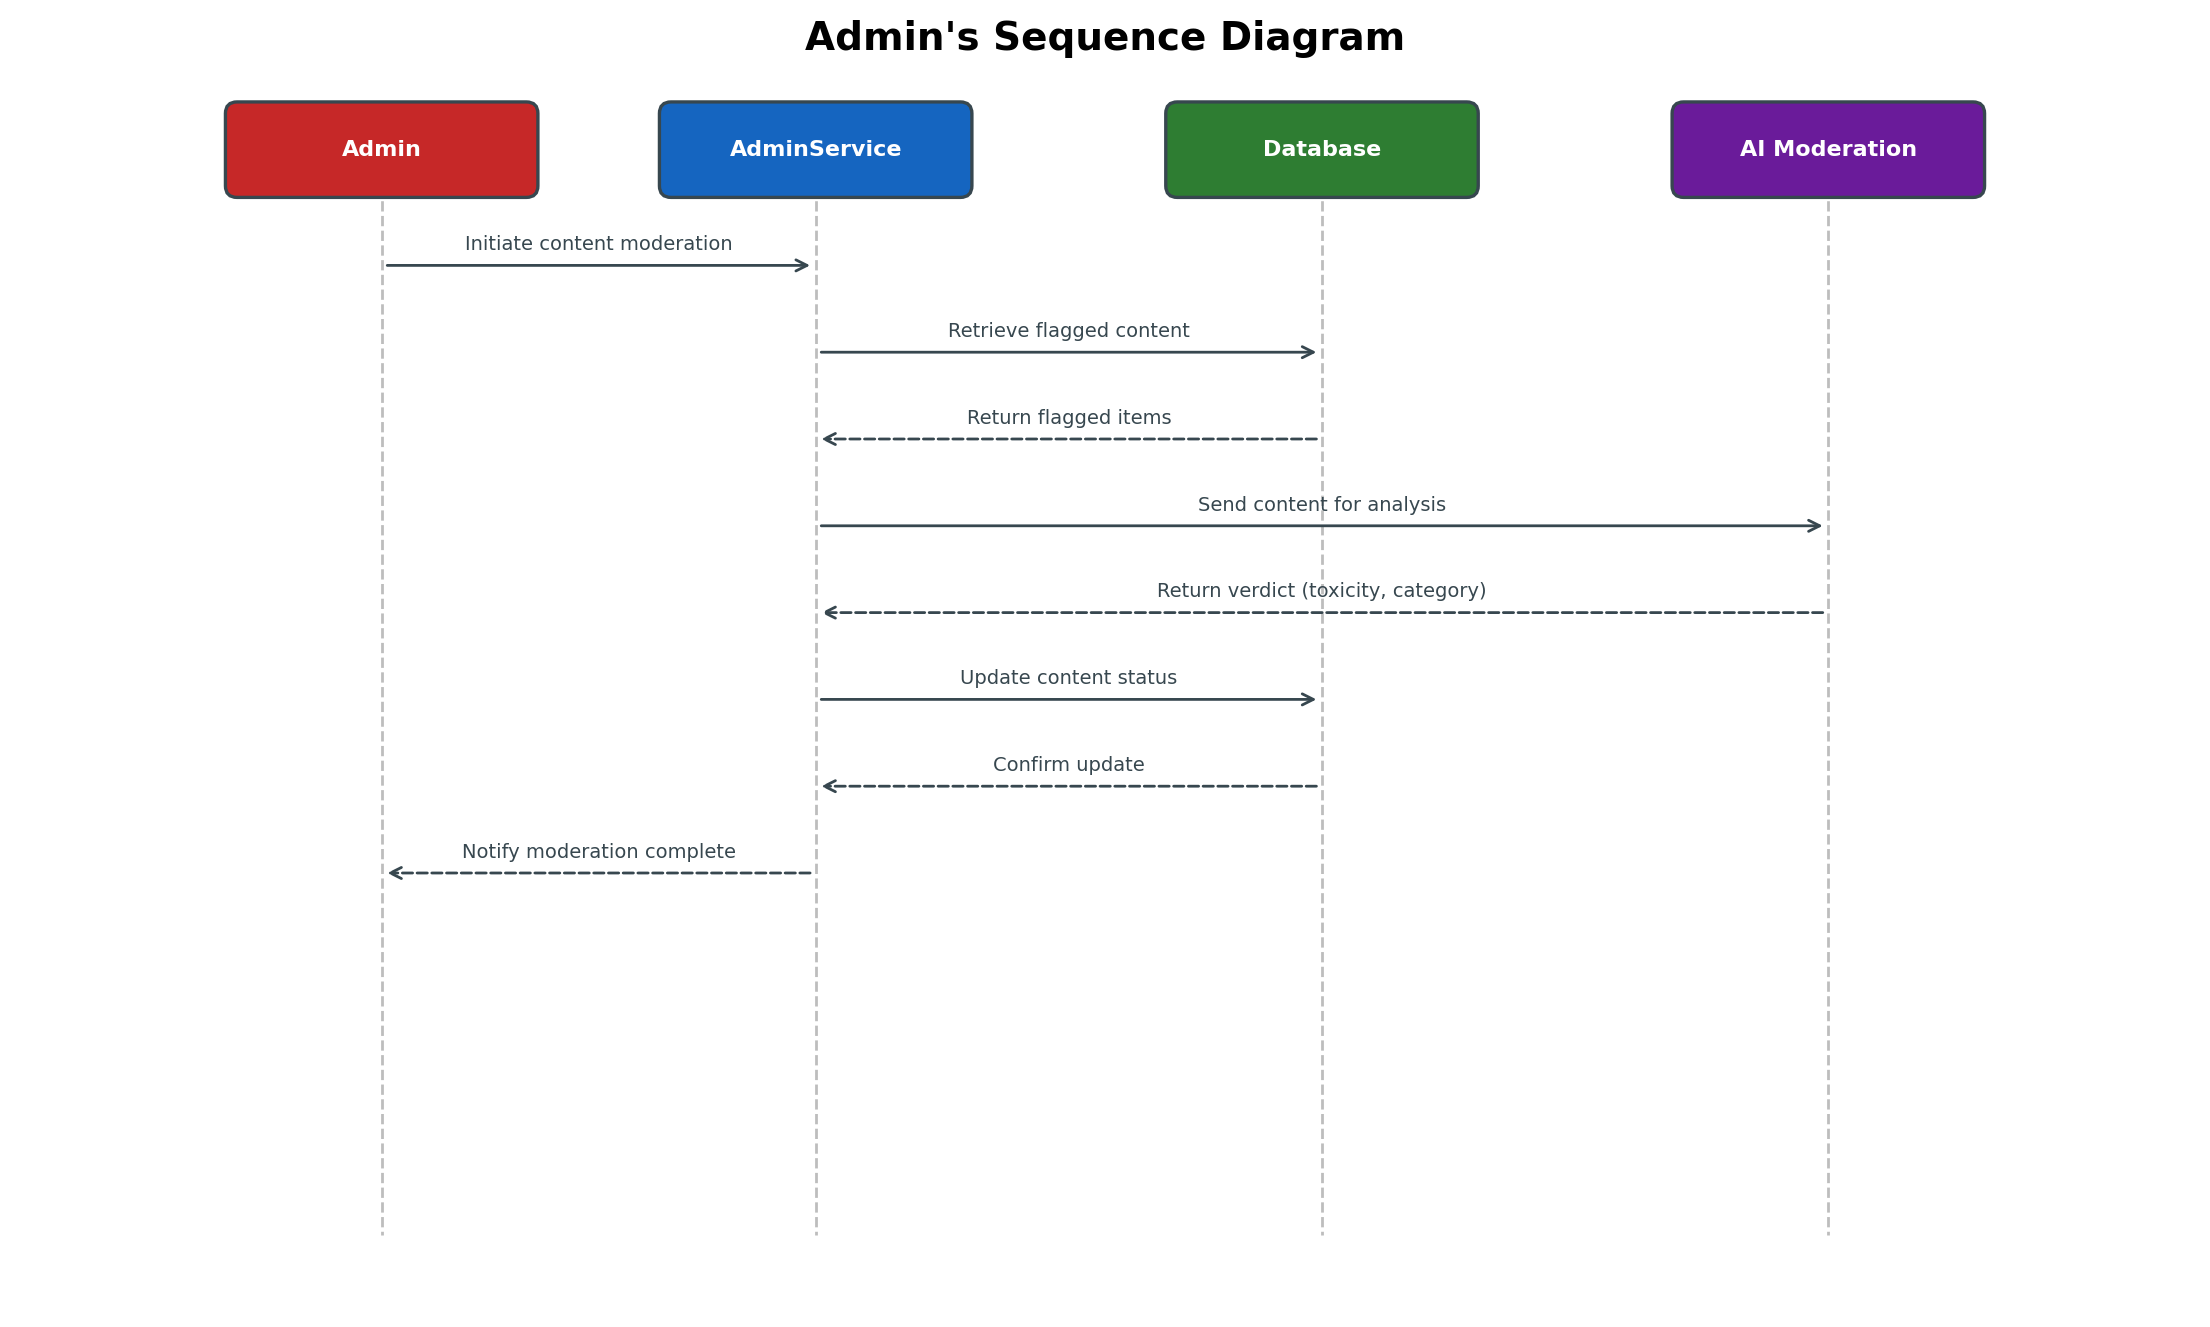
\includegraphics[width=0.9\textwidth]{images/admin-sequence.png}
\caption{Admin's Sequence Diagram}
\label{fig:admin-sequence}
\end{figure}

The admin's sequence diagram illustrates how flagged content is moderated through interaction among the Admin, AdminService, Database, and the AI moderation engine. The process starts when the Admin initiates content moderation. The AdminService retrieves the flagged content from the database, then sends it to the AI moderation engine for analysis. After analyzing the content, the engine returns a verdict to the AdminService. Based on this verdict, the AdminService updates the content status in the database. Once the update is complete, the system notifies the Admin that the action has been completed.

\subsection{Creator's Sequence Diagram}

\begin{figure}[H]
\centering
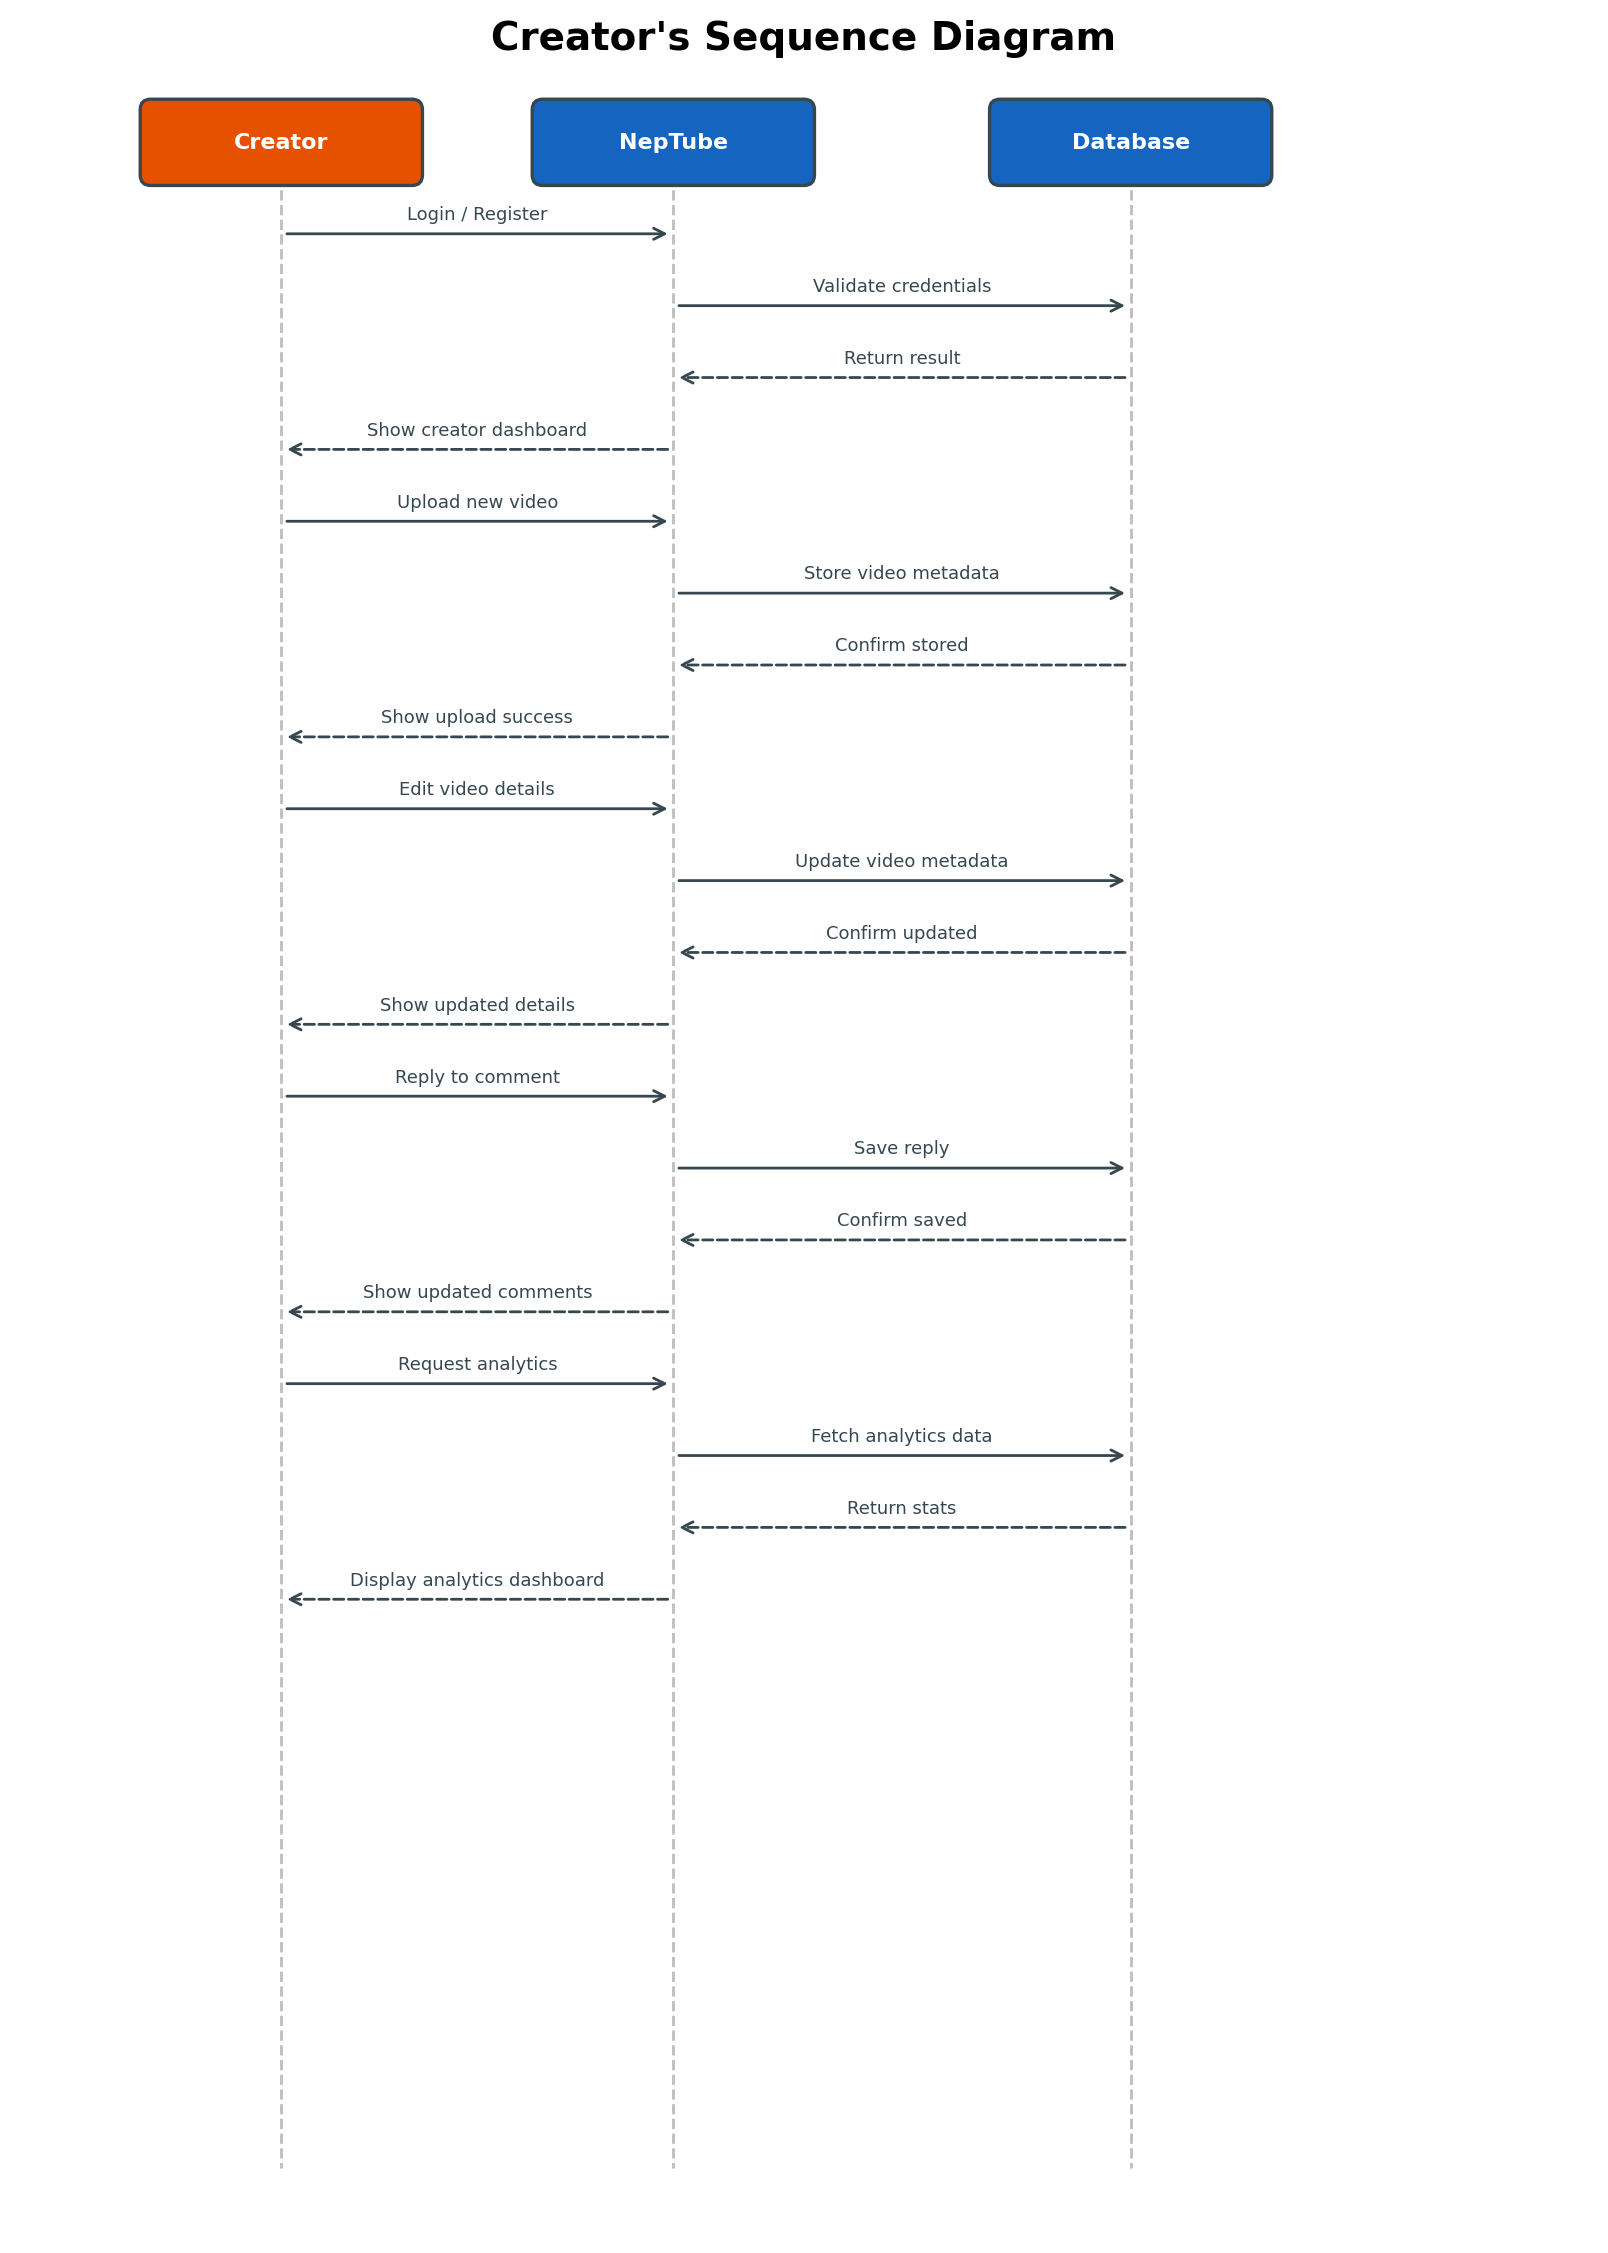
\includegraphics[width=0.9\textwidth]{images/creator-sequence.png}
\caption{Creator's Sequence Diagram}
\label{fig:creator-sequence}
\end{figure}

The creator's sequence diagram illustrates the interactions between a content creator, the NepTube platform, and its database, focusing on video management, viewer engagement, and analytics. The process begins when the creator logs in or registers, prompting NepTube to validate credentials through the database and return a success or failure message. Upon successful login, the system displays the creator's dashboard. The creator can then add a new video, which is sent to NepTube and updated in the database. A confirmation is returned, followed by a success or failure message shown to the creator. If needed, the creator can edit the details of an already uploaded video, with the changes being updated in the database and confirmed back to the creator. Next, the creator can engage with viewers by replying to comments; these replies are updated in the comment section and confirmed by the database, leading to the display of the updated comment section. Finally, the creator may choose to view analytics such as channel statistics and video performance data. This request prompts NepTube to fetch the relevant data from the database, and once retrieved, the data is displayed to the creator. This entire sequence ensures seamless content management and audience interaction for creators on the platform.

\section{System Architecture}

The system architecture of NepTube follows a layered design pattern, separating concerns into distinct tiers for maintainability, scalability, and modularity. The architecture comprises four primary layers:

\begin{itemize}[leftmargin=2cm]
  \item \textbf{Presentation Layer:} Built with Next.js \cite{vercel2024nextjs} and React 19 \cite{react2024docs}, this layer handles all user interactions. Tailwind CSS \cite{tailwindcss2024docs} and Radix UI \cite{radixui2024docs} primitives provide responsive, accessible styling.
  \item \textbf{Application Layer:} tRPC \cite{trpc2024docs} API routes running on the Bun \cite{bun2024docs} runtime handle business logic. Clerk \cite{clerk2024docs} manages authentication, while UploadThing \cite{uploadthing2024docs} handles file uploads.
  \item \textbf{Data Layer:} PostgreSQL \cite{postgresql2025docs} (hosted on Neon \cite{neon2024docs}) stores all persistent data, accessed through Drizzle ORM \cite{drizzle2024docs} for type-safe schema definitions and queries.
  \item \textbf{AI/ML Services:} External APIs including Pollinations \cite{pollinations2024api} for NLP text generation and Replicate \cite{replicate2024whisper} for Whisper~v3 transcription \cite{radford2023whisper} power intelligent features.
\end{itemize}

\begin{figure}[H]
\centering
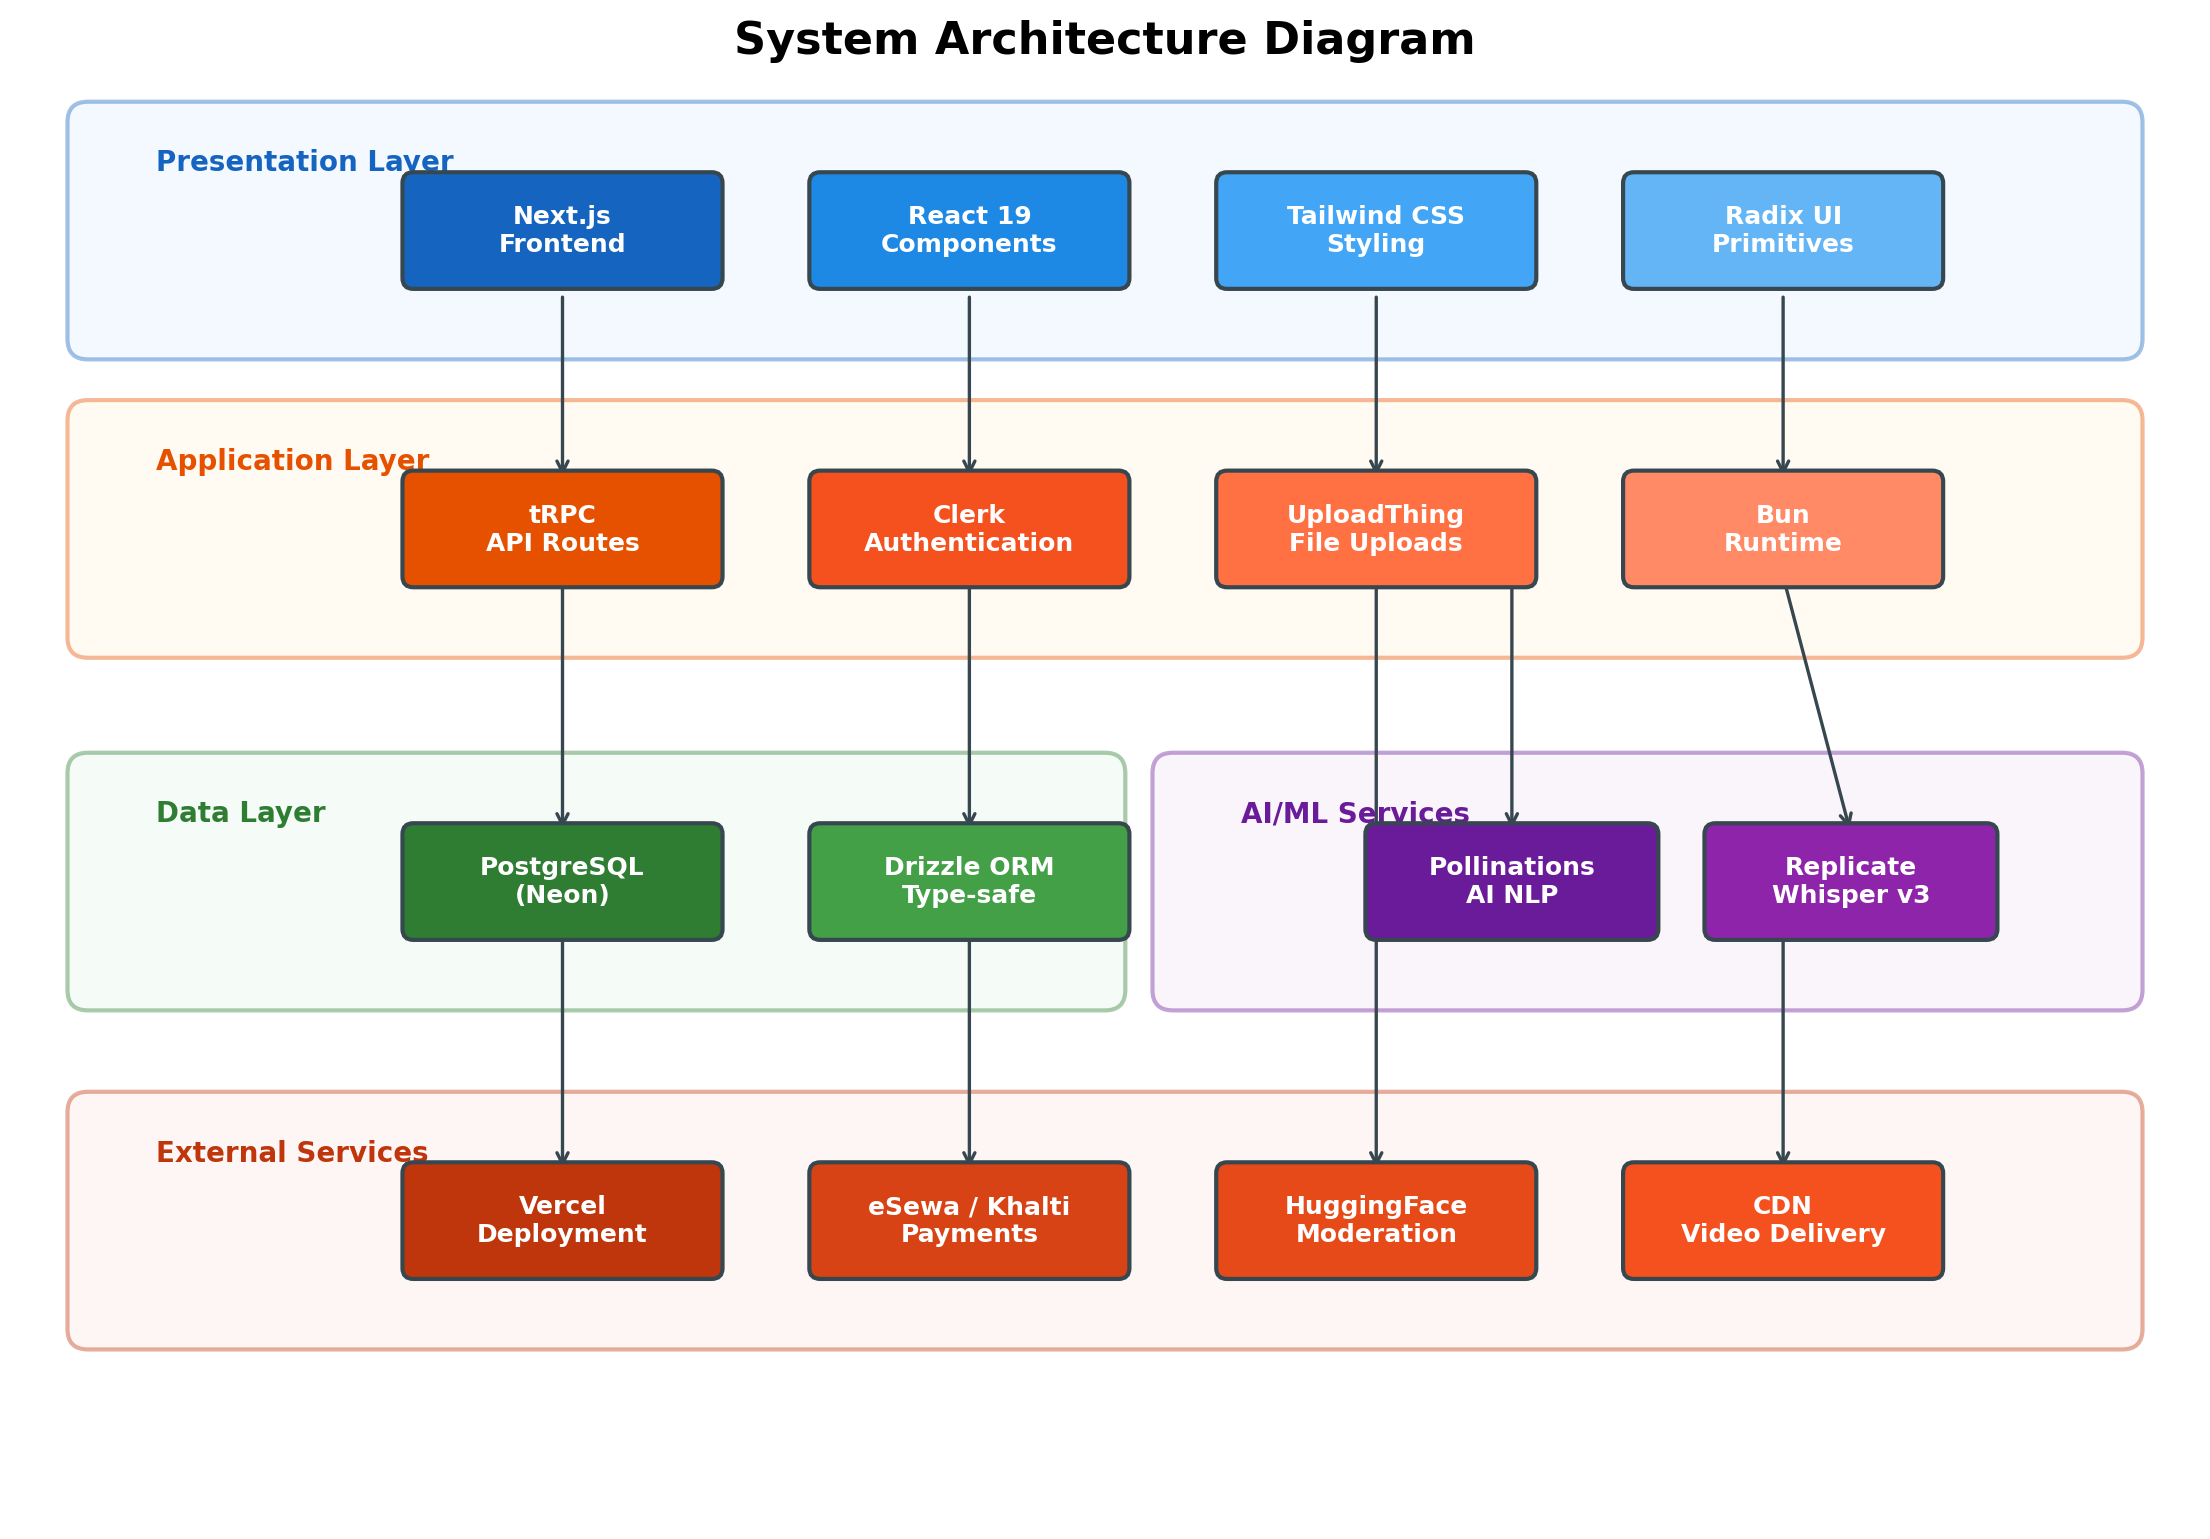
\includegraphics[width=0.90\textwidth]{images/system-architecture.png}
\caption{System Architecture Diagram}
\label{fig:system-architecture}
\end{figure}

The layered architecture ensures that changes in one layer---such as switching the AI provider or database host---do not affect other layers. Communication between the frontend and backend is fully type-safe through tRPC, eliminating runtime type errors and improving developer productivity.

\section{Entity Relationship (ER) Diagram}

The Entity Relationship diagram illustrates the database schema and the relationships between core entities in the NepTube platform. The system uses a relational database (PostgreSQL) with the following principal entities:

\begin{itemize}[leftmargin=2cm]
  \item \textbf{Users:} Stores user profiles, authentication references, roles, subscription tiers, and ban status.
  \item \textbf{Videos:} Contains video metadata, URLs, view counts, AI-generated fields (summary, transcript, content DNA), and premium access flags.
  \item \textbf{Comments:} Holds user comments with parent references for threading, along with ML-powered sentiment and toxicity scores.
  \item \textbf{Subscriptions:} Records channel subscriptions between users (subscriber--channel relationship).
  \item \textbf{Playlists \& PlaylistVideos:} Manages user-created playlists and their ordered video entries.
  \item \textbf{VideoLikes:} Tracks likes and dislikes on videos with a boolean flag.
  \item \textbf{WatchHistory:} Logs viewing sessions with timestamps and watch duration for recommendation training.
  \item \textbf{Notifications:} Stores user notifications with type, read status, and references to triggering entities.
  \item \textbf{Reports:} Records content reports filed by users with status tracking and admin resolution notes.
\end{itemize}

\begin{figure}[H]
\centering
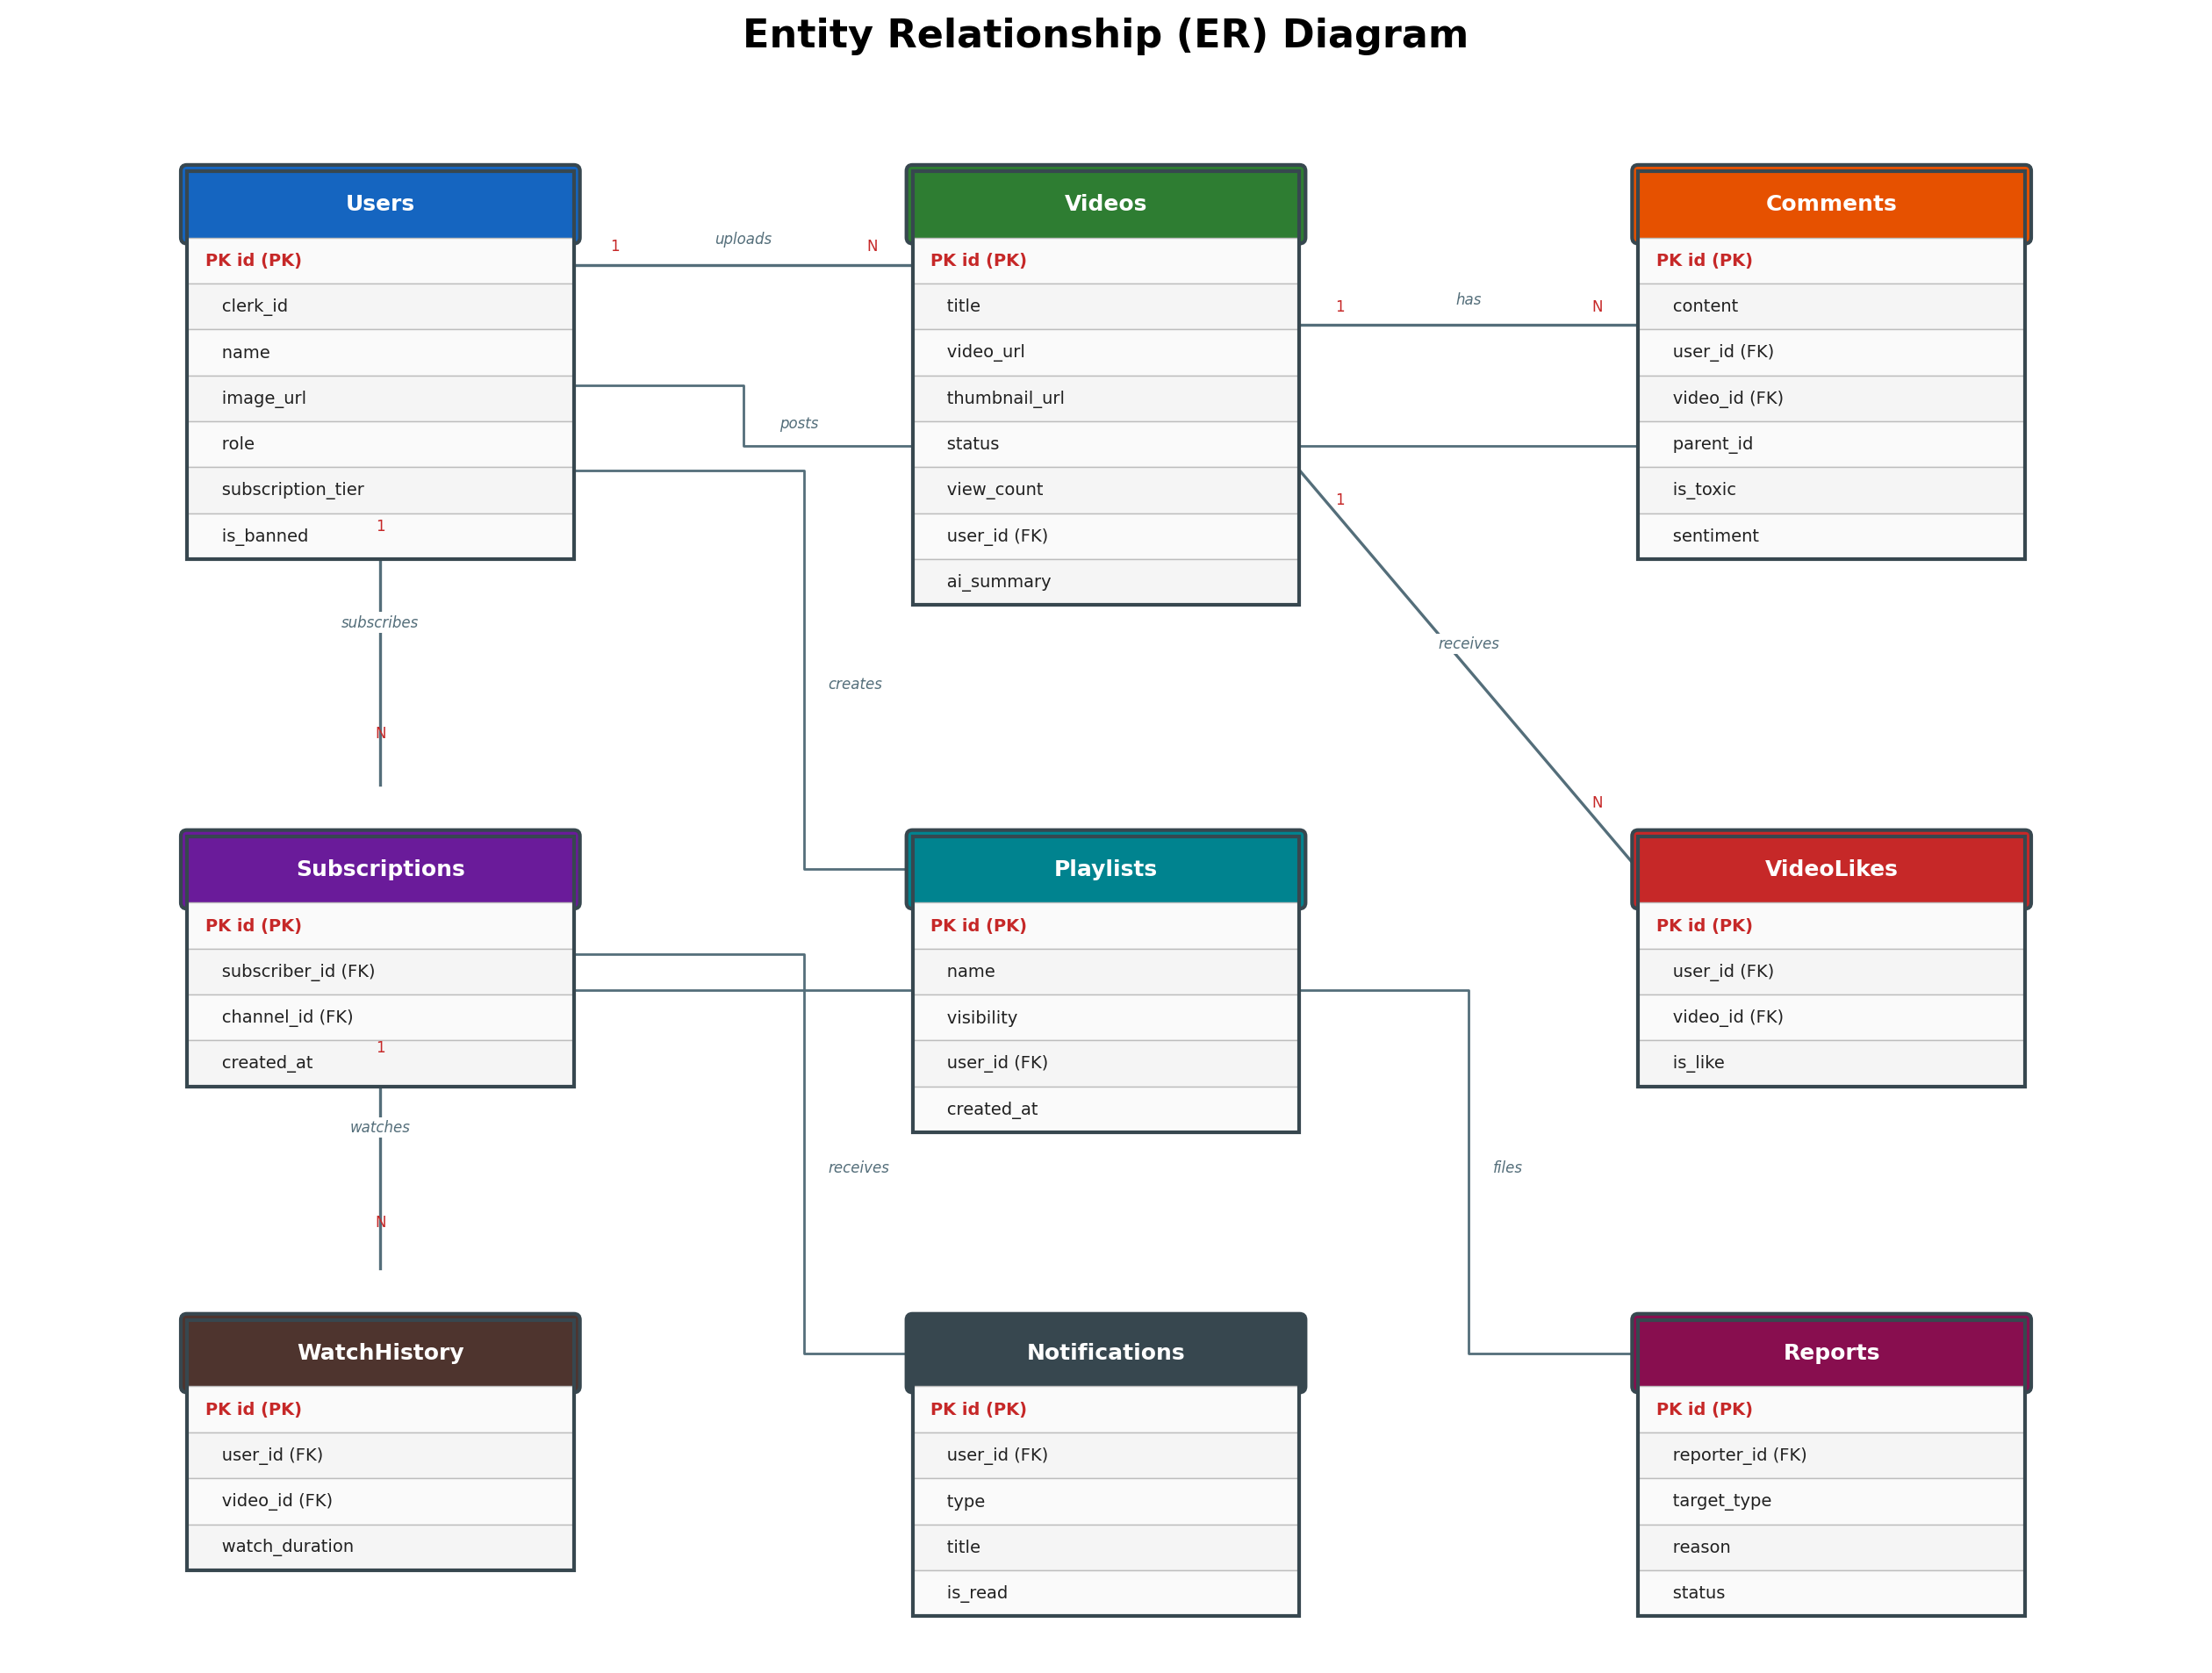
\includegraphics[width=0.90\textwidth]{images/er-diagram.png}
\caption{Entity Relationship (ER) Diagram}
\label{fig:er-diagram}
\end{figure}

All foreign key relationships use cascading deletes to maintain referential integrity. Unique indexes are applied on composite keys (e.g., user--video pairs for likes and watch history) to prevent duplicate records and ensure data consistency.

\section{Data Flow Diagram}

The Data Flow Diagram (DFD) Level~0 provides a context-level overview of the NepTube system, showing the flow of data between external entities and the central process. The diagram identifies the following external entities that interact with the system:

\begin{itemize}[leftmargin=2cm]
  \item \textbf{Viewer:} Sends requests to watch, like, comment, and subscribe; receives videos, recommendations, and notifications.
  \item \textbf{Content Creator:} Uploads videos, edits metadata; receives analytics data and AI-generated thumbnails and titles.
  \item \textbf{Admin:} Initiates moderation actions and user management; receives reports and platform analytics.
  \item \textbf{PostgreSQL Database:} Serves as the persistent data store for all entities and relationships.
  \item \textbf{AI/ML Services:} Processes content for analysis, recommendations, transcription, and moderation verdicts.
  \item \textbf{Payment Gateway:} Handles premium subscription payments through eSewa \cite{esewa2024}, Khalti \cite{khalti2024}, and international gateways.
\end{itemize}

\begin{figure}[H]
\centering
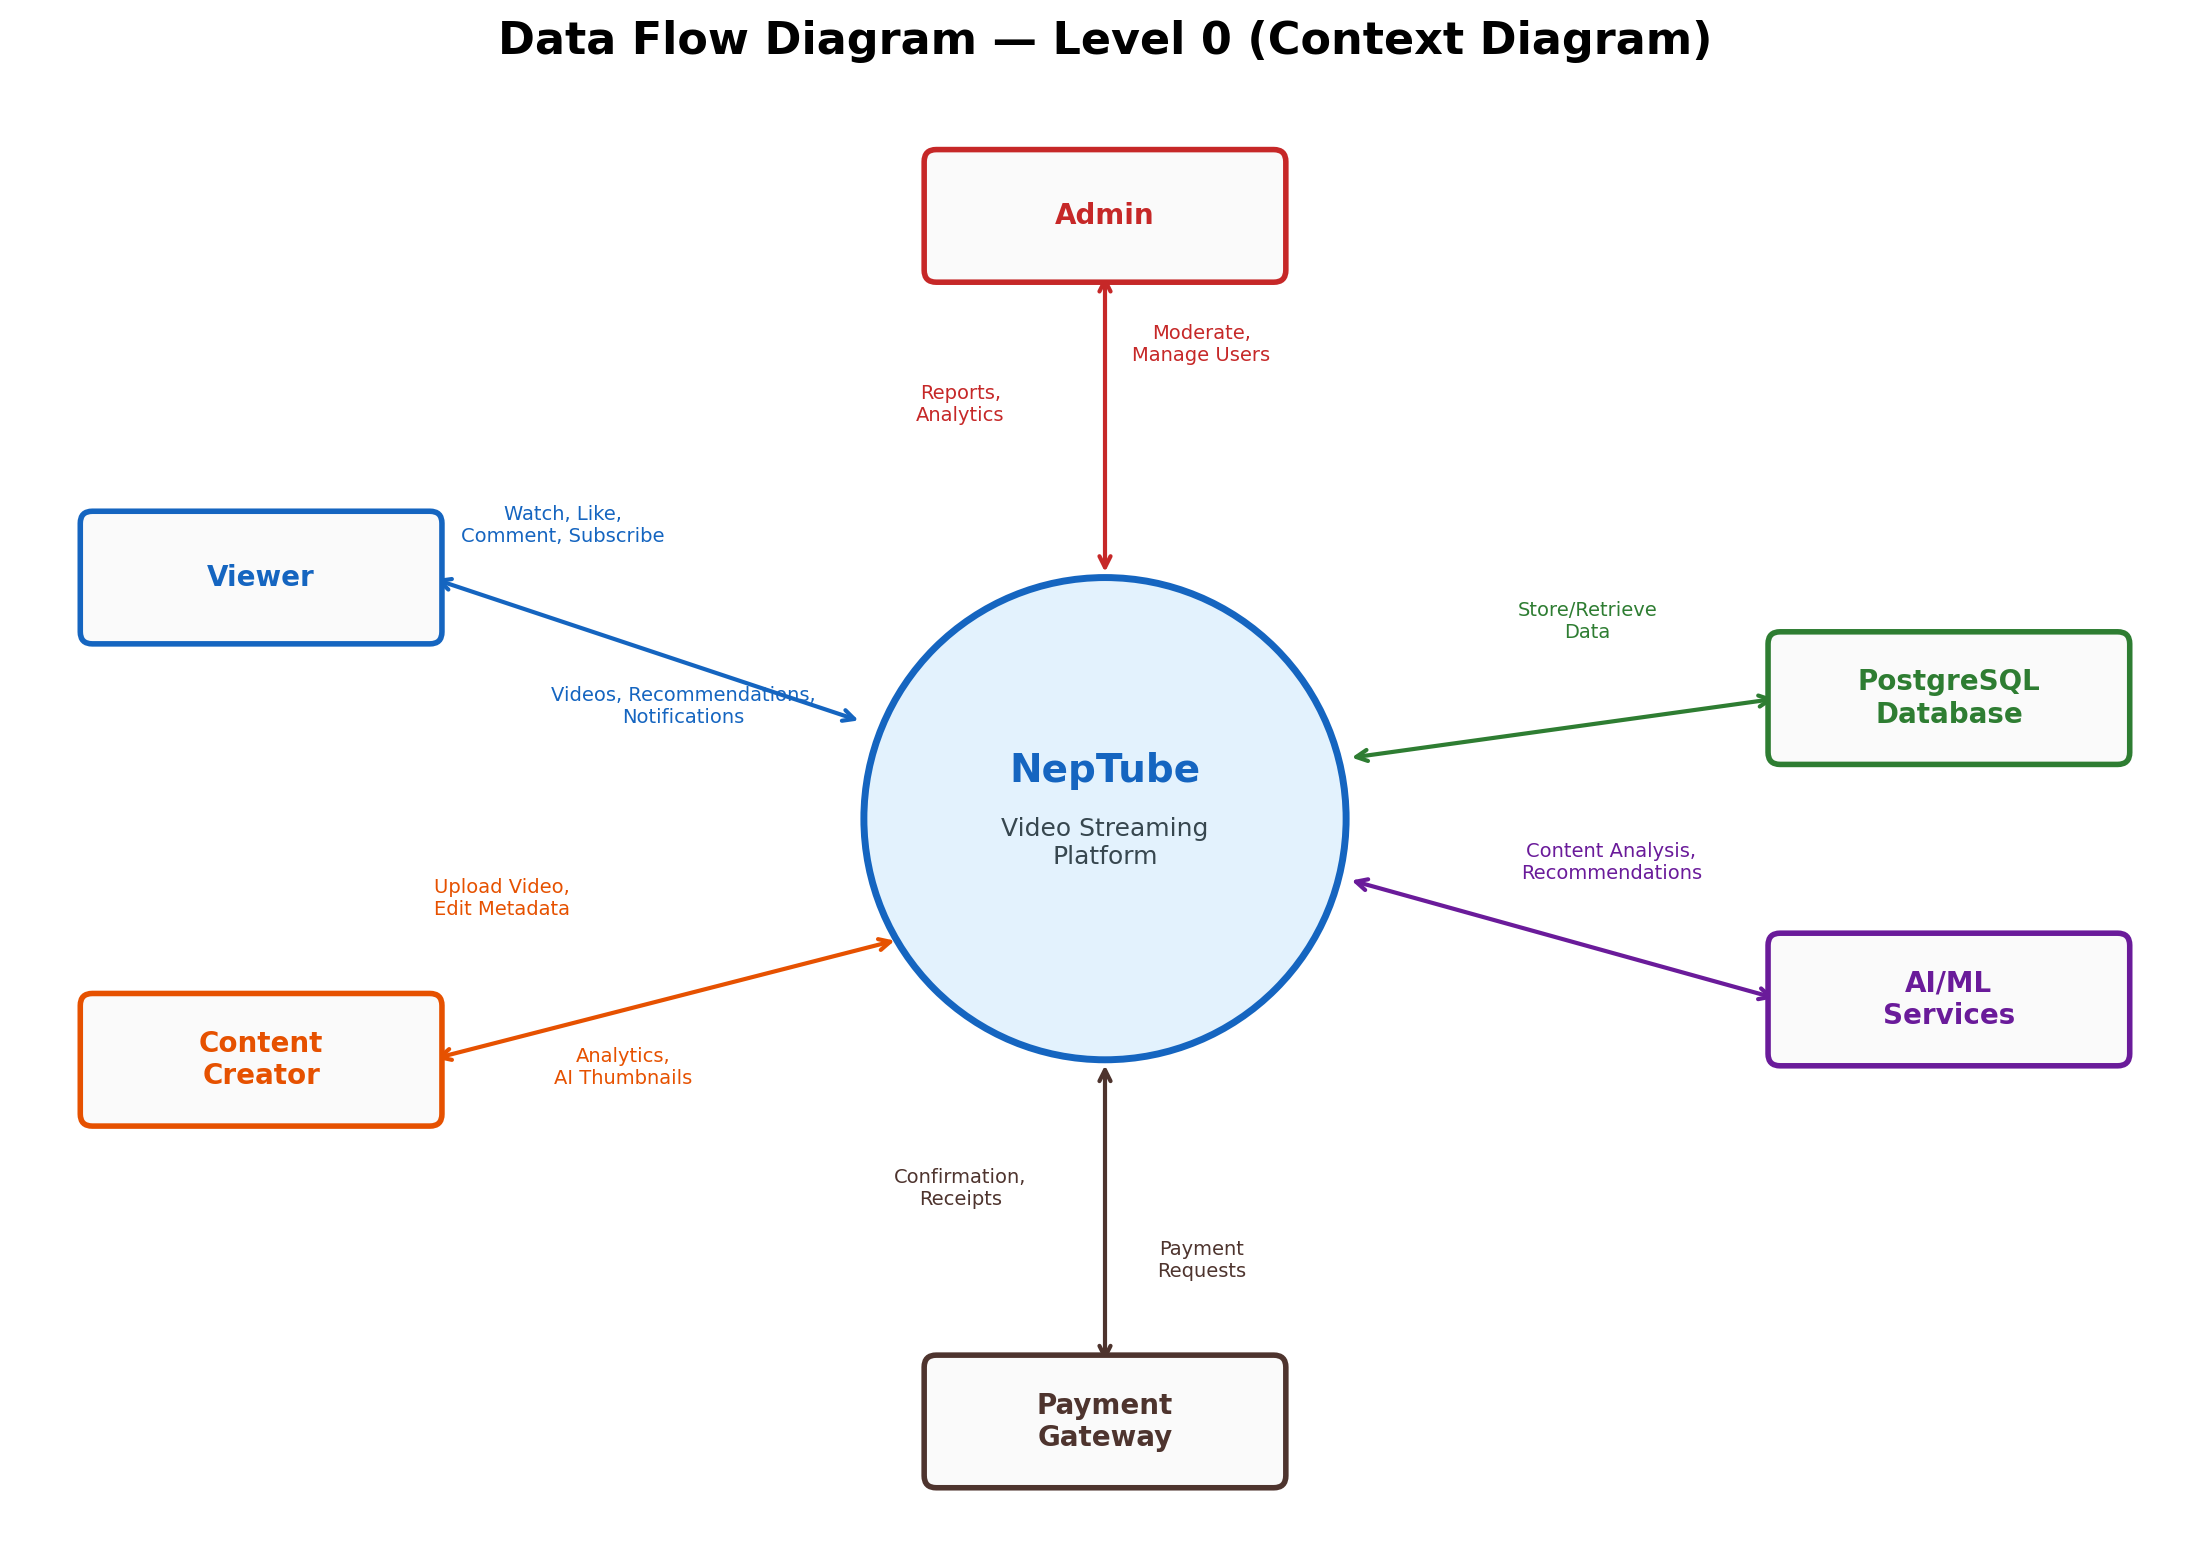
\includegraphics[width=0.85\textwidth]{images/dfd-diagram.png}
\caption{Data Flow Diagram --- Level 0 (Context Diagram)}
\label{fig:dfd-level0}
\end{figure}

The context diagram clearly delineates the system boundary, showing NepTube as a central process that mediates all data flows between users, databases, AI services, and payment providers.

\section{Technology Stack}

The NepTube project utilizes a modern and robust technology stack to ensure scalability, performance, and ease of development. The main components are as follows:

\begin{itemize}[leftmargin=2cm]
  \item \textbf{Frontend:} Next.js \cite{vercel2024nextjs} with React 19 \cite{react2024docs} and TypeScript \cite{typescript2024docs} for building interactive and responsive user interfaces, styled with Tailwind CSS \cite{tailwindcss2024docs} and accessible Radix UI primitives \cite{radixui2024docs}.
  \item \textbf{Backend:} Next.js API routes and tRPC \cite{trpc2024docs} for end-to-end type-safe server logic, running on the Bun runtime \cite{bun2024docs}.
  \item \textbf{Database:} PostgreSQL \cite{postgresql2025docs} hosted on Neon \cite{neon2024docs}, managed through Drizzle ORM \cite{drizzle2024docs} for type-safe schema and queries.
  \item \textbf{Authentication:} Clerk \cite{clerk2024docs} for secure user authentication and profile management.
  \item \textbf{File Uploads:} UploadThing \cite{uploadthing2024docs} for efficient video and image uploads.
  \item \textbf{AI Integration:} Pollinations \cite{pollinations2024api} for NLP text generation, Replicate \cite{replicate2024whisper} for Whisper~v3 transcription \cite{radford2023whisper}, and AI-powered content moderation \cite{risch2020toxic}.
  \item \textbf{Accessibility:} UI components follow WCAG 2.2 guidelines \cite{w3c2023wcag} through Radix UI accessible primitives.
  \item \textbf{Testing:} Manual testing across browsers and devices to ensure reliability and compatibility.
\end{itemize}
